\documentclass[a4paper]{cernatsnote}
\usepackage{graphicx}
\usepackage{listings}
\usepackage{caption}
\usepackage{listings}
\usepackage{parskip}
\usepackage{hyperref}
\usepackage{caption}
\usepackage{subcaption}


\usepackage[usenames,dvipsnames]{xcolor}

\definecolor{dkgreen}{rgb}{0,0.6,0}
\definecolor{gray}{rgb}{0.5,0.5,0.5}
\definecolor{mauve}{rgb}{0.58,0,0.82}
\definecolor{Brown}{cmyk}{0,0.81,1,0.60}
\definecolor{OliveGreen}{cmyk}{0.64,0,0.95,0.40}
\definecolor{CadetBlue}{cmyk}{0.62,0.57,0.23,0}

\definecolor{amber}{rgb}{1.0, 0.49, 0.0}
\definecolor{azure}{rgb}{0.0, 0.5, 1.0}
\definecolor{brandeisblue}{rgb}{0.0, 0.44, 1.0}
\definecolor{fluorescentpink}{rgb}{1.0, 0.08, 0.58}
\definecolor{lime}{rgb}{0.0, 1.0, 0.0}

\lstset{ 
	backgroundcolor	=	\color{white},  				% choose the background color; you must add \usepackage{color} or \usepackage{xcolor}
	basicstyle		=	\footnotesize,       				% the size of the fonts that are used for the code
	%basicstyle	=	\normalsize,
	breakatwhitespace=	false,       					% sets if automatic breaks should only happen at whitespace
	breaklines		=	true,               				% sets automatic line breaking
	captionpos		=        b,                   				% sets the caption-position to bottom
	commentstyle	=	\color{dkgreen},  				% comment style
	% deletekeywords	=	{...},        					% if you want to delete keywords from the given language
	escapeinside	=	{\%*}{*)},         				% if you want to add LaTeX within your code
	%extendedchar	=	true,              				% lets you use non-ASCII characters; for 8-bits encodings only, does not work with UTF-8
	frame			=	ltrb,                  				% adds a frame around the code
	framesep		=	5pt,
	identifierstyle	=	\ttfamily \color{black}\bfseries,
	keywordstyle	=	\ttfamily \color{blue},      		% keyword style
	language		=	Bash,                				% the language of the code
	morekeywords	=	{*,...},           				% if you want to add more keywords to the set
	numbers			=	left,                   				% where to put the line-numbers; possible values are (none, left, right)
	numbersep		=	5pt,                  				% how far the line-numbers are from the code
	numberstyle		=	\tiny\color{gray},  				% the style that is used for the line-numbers
	rulecolor		=	\color{black},        				% if not set, the frame-color may be changed on line-breaks within not-black text (e.g. comments (green here))
	showspaces		=	false,               				% show spaces everywhere adding particular underscores; it overrides 'showstringspaces'
	showstringspaces	=	false,         					% underline spaces within strings only
	showtabs		=	false,                 				% show tabs within strings adding particular underscores
	stepnumber		=	2,                  				% the step between two line-numbers. If it's 1, each line will be numbered
	stringstyle		=	\ttfamily\color{gray},      		% string literal style
	tabsize			=	2,                      				% sets default tabsize to 2 spaces
	title			=	\lstname                  				% show the filename of files included with \lstinputlisting; also try caption instead of title
}

% Base classes
\lstset{
	emph		=	{mkdir, cp, ln, ssh, module, git, curl, make},
	emphstyle		= 	\ttfamily \color{blue}
}

% User classes
\lstset{
	emph		=	{[2]User_Class, myMADInterface},
	emphstyle		= 	{[2]\ttfamily \color{amber}}
}

% Functions
\lstset{
	emph		=	{[3]Function, TreatTypeAsDrift},
	emphstyle		= 	{[3]\ttfamily \color{fluorescentpink}}
}

% Units
\lstset{
	emph		={[4]Unit, km, TeV, eV, meter}, emphstyle	=	{[4]\ttfamily \color{lime}}
}


\email{haroon.rafique@cern.ch}

\title{PTC-PyORBIT SIS18 Benchmark}
\documentlabel{CERN-ATS-Note-2018-??? TECH}

\author{Haroon Rafique / BE-ABP}
\keywords{PyORBIT, Space Charge, SIS18, Benchmark}
\makeindex

\def \gsiSISpage {\href{https://web-docs.gsi.de/~giuliano/research_activity/trapping_benchmarking/main.html}{https://web-docs.gsi.de/~giuliano/research\_activity/trapping\_benchmarking/main.html}}
\def \hbgithub {\href{https://github.com/hannes-bartosik/py-orbit}{https://github.com/hannes-bartosik/py-orbit.git}}
\def \ptcgithub {\href{https://github.com/jbcern/PTC/tree/analytical-space-charge-acceleration}{https://github.com/jbcern/PTC.git}}
\def \franchettipaper {\href{https://web-docs.gsi.de/~giuliano/publications/reports_not_on_web/HB2006_THBW01.pdf}}

\begin{document}
	
\maketitle % this produces the title block

\begin{abstract}
	The effects of space charge on particle beams in accelerators are many and complex. Interplay exists between space charge and other effects such as the electron cloud. Space charge is dependent on the beam distribution longitudinally and transversely, the structure and layout of the particle accelerator in which the beam is maintained, and the complex dynamics that may include other coherent and incoherent effects.
	
	As such, comparing a space charge simulation with experiment or other simulation tools is difficult. Giuliano Franchetti, together with Ingo Hofmann and Shinji Machida compared the space charge simulation tools MICROMAP and SIMPSONS using the SIS18 accelerator in GSI Darmstadt. 	
	
	Giuliano Franchetti's SIS18 benchmark has been performed with the PTC-PyORBIT code, the steps taken to achieve this, and the results, are detailed in this report.
\end{abstract}

%%%%%%%%%%%%%%%%%%----------------------------------------------------------------------------------------
%% INTRODUCTION %%
%%%%%%%%%%%%%%%%%%----------------------------------------------------------------------------------------	
\section{Introduction}
\label{sec:intro}

Details of the SIS18 benchmark can be found at:
\gsiSISpage

These instructions are repeated and expanded upon here. 
	
%% Setup %%
%%%%%%%%%%%%%%------------------------------------------------------------------------------------------			
\section{Simulation Setup}

\subsection{SIS18 Parameters}
The parameters in table~\ref{tab:parameters16} are used in steps 1 - 6, and the changes in table~\ref{tab:parameters79} are used in steps 7 - 9.

\begin{table}
	\begin{center}
		\begin{tabular}[!b]{|l|c|c|c|}
			\hline
			\textbf{Parameter} & \textbf{Symbol} & \textbf{Value} & \textbf{Unit} \\
			\hline
			\textbf{Sextupole Strength} & $K_2$ & 0.2 & $m^{-2}$ \\
			\textbf{Maximum Tuneshift} & $\Delta Q_x$ & 0.1 & $-$ \\
			\textbf{Horizontal Transverse Size (rms)} & $X_{rms}$ & 5 & $mm$ \\
			\textbf{Vertical Transverse Size (rms)} & $Y_{rms}$ & 5 & $mm$ \\
			\textbf{Longitudinal Size (rms)} & $Z_{rms}$ & 40.35 & $m$ \\
			\textbf{Horizontal Geometric Emittance (2 $\sigma$)} & $\epsilon_x$ & 12.57 & $mm~mrad$ \\
			\textbf{Vertical Geometric Emittance (2 $\sigma$)} & $\epsilon_y$ & 9.30 & $mm~mrad$ \\
			\textbf{One Synchrotron Oscillation} & $N_{synch}$ & 15000 & $turns$ \\
			\textbf{Bunch Length (4 $\sigma_z$)} & $\tau$ & 3472.7 & $ns$ \\
			\textbf{Kinetic Energy} & $E_k$ & 11.4 & $MeV/u$ \\
			\textbf{Transition Gamma} & $\gamma_t$ & 5 & $-$ \\
			\textbf{Momentum Spread (3 $\sigma$)} & $\frac{\Delta p}{p}$ & 2.5$\cdot 10^{-4}$ & $-$ \\
			\textbf{Sextupole Strength} & $K_2$ & 0.2 & $m^{-2}$ \\
			\hline
		\end{tabular}
		\caption{Parameters used for the SIS18 benchmark steps 1 - 6.}
		\label{tab:parameters16}
	\end{center}
\end{table}

\begin{table}
	\begin{center}amplitude detuning
		\begin{tabular}[!b]{|l|c|c|c|}
			\hline
			\textbf{Parameter} & \textbf{Symbol} & \textbf{Value} & \textbf{Unit} \\
			\hline
			\textbf{Longitudinal Size (rms)} & $Z_{rms}$ & 2.69 & $m$ \\
			\textbf{One Synchrotron Oscillation} & $N_{synch}$ & 1000 & $turns$ \\
			\textbf{Bunch Length (4 $\sigma_z$)} & $\tau$ &  231.51 & $ns$ \\
			\hline
		\end{tabular}
		\caption{Parameter changes used for the SIS18 benchmark steps 7 - 9.}
		\label{tab:parameters79}
	\end{center}
\end{table}

\subsection{PTC-PyORBIT Setup}

The PyORBIT version used was pulled from Hannes Bartosik's GitHub repository in March 2018. It can be found at: \hbgithub 
The PTC version used was pulled from Jean-Baptiste Lagrange's GitHub repository in March 2018. It can be found at: \hbgithub 

It is important to note that in order to ensure that PTC uses the correct units, the time.ptc file must be included in the PTC-PyORBIT simulation. The file contents are shown in Fig.~\ref{fig:ptc_time}.

\begin{figure}
	\begin{lstlisting}[language=bash, belowskip=-3\medskipamount]
	select layout
	1
	+time
	set orbit state
	return
	\end{lstlisting}
	\caption{time.ptc file required to use correct units in PTC.}
	\label{fig:ptc_time}
\end{figure}



\newpage

\section{Step 1: Benchmarking of the phase space}

The first step is to confirm that the phase space near the 3rd order resonance has the same topology for all codes. We check the orbits up to the border of stability (dynamic aperture). For this test the tunes are $Q_x$ = 4.338, $Q_y$ = 3.2, the Poincar\'{e} section is plot at the beginning of the SIS18 lattice. 

\begin{figure}
        \centering
        \begin{subfigure}{.5\textwidth}
          \centering
          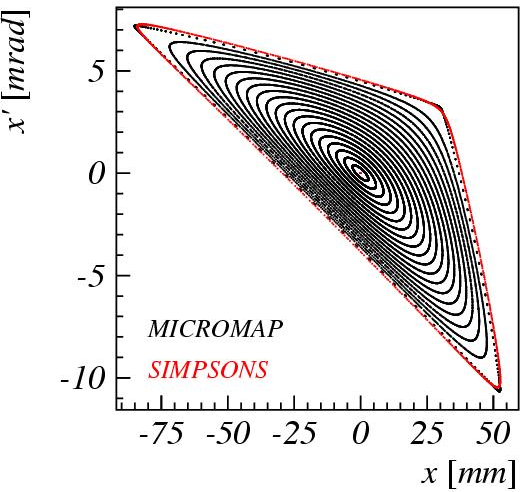
\includegraphics[width=\textwidth]{Step1_phase-space.png}
          \caption{MICROMAP and SIMPSONS.}
          \label{fig:step1_m}
        \end{subfigure}~~~~~~
        \begin{subfigure}{.5\textwidth}
          \centering
          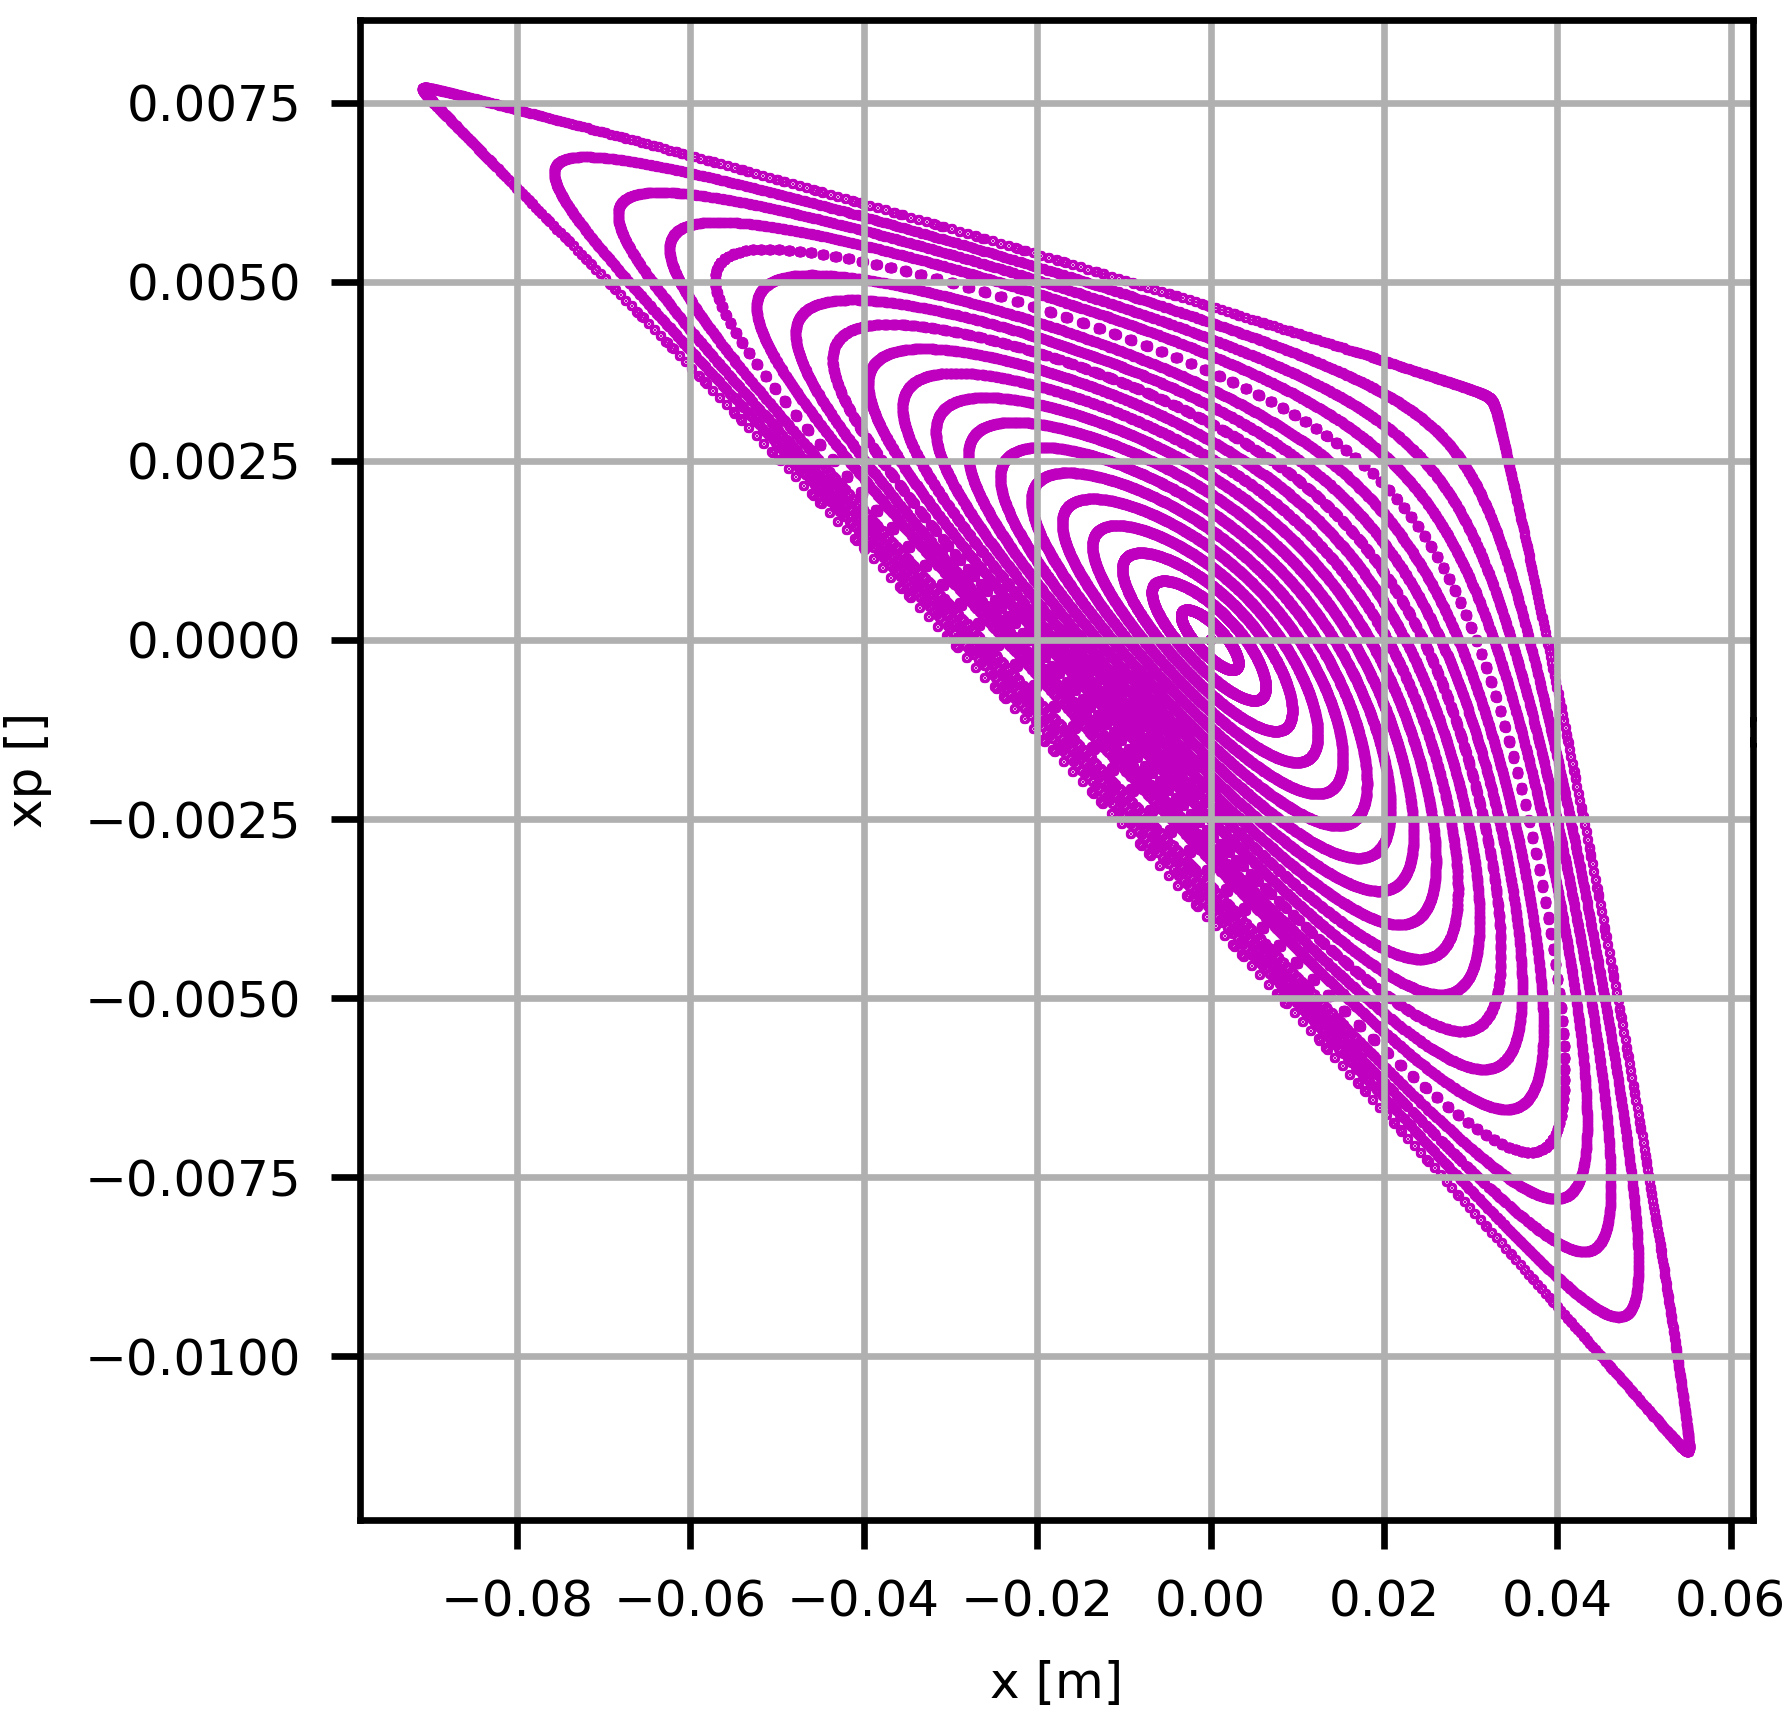
\includegraphics[width=\textwidth]{Step1_phase-space_PO.png}
          \caption{PTC-PyORBIT.}
          \label{fig:step1_po}
        \end{subfigure}
        \caption{Step1: Phase space with sextupole on and no space charge.}
        \label{fig:step1}
\end{figure}

\section{Step 2: Tunes with sextupole off}

The second step is to benchmark the dependence of a test particle tune from its amplitude. The amplitude of the particle is here meant as the effective maximum amplitude that the particle can have in one betatron oscillation. The particle coordinates of the test particles are: $x_0$ = 0, ..., 4 $\sigma_x$, $p_{x0}$ = $y_0$ = $p_{y0}$ = 0. The particle amplitude is therefore $x = \sqrt{\beta_x \gamma_x} x_0$. The same definition applies to the y amplitude. The lattice sextupole is off. As the bunch space charge is maximum at the center of the bunch, the test is performed keeping the particle at z = 0. The bare tunes are are $Q_x$ = 4.338, $Q_y$ = 3.2. The tunes are computed with a fourier transform of the motion of a test particle over 1024 turns. 
The factor $\sqrt{\beta_x \gamma_x}$ is that required to transform the initial particle (with co-ordinate ($x,xp$) = (0 - 4 $\sigma_x$, 0)) to it's maximum amplitude in $x$, as $x_0 = \sqrt{\frac{\epsilon_x}{\gamma_x}}$, and the maximum amplitude is $\sqrt{\beta_x \epsilon_x}$.


\begin{figure}
        \centering
        \begin{subfigure}{.5\textwidth}
          \centering
          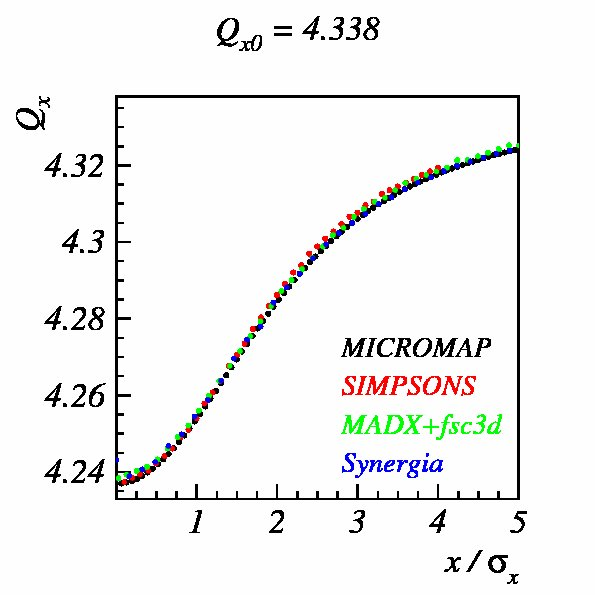
\includegraphics[width=\textwidth]{Step2_tune_x.png}
          \caption{MICROMAP and SIMPSONS.}
          \label{fig:step2H_m}
        \end{subfigure}~~~~~~
        \begin{subfigure}{.5\textwidth}
          \centering
          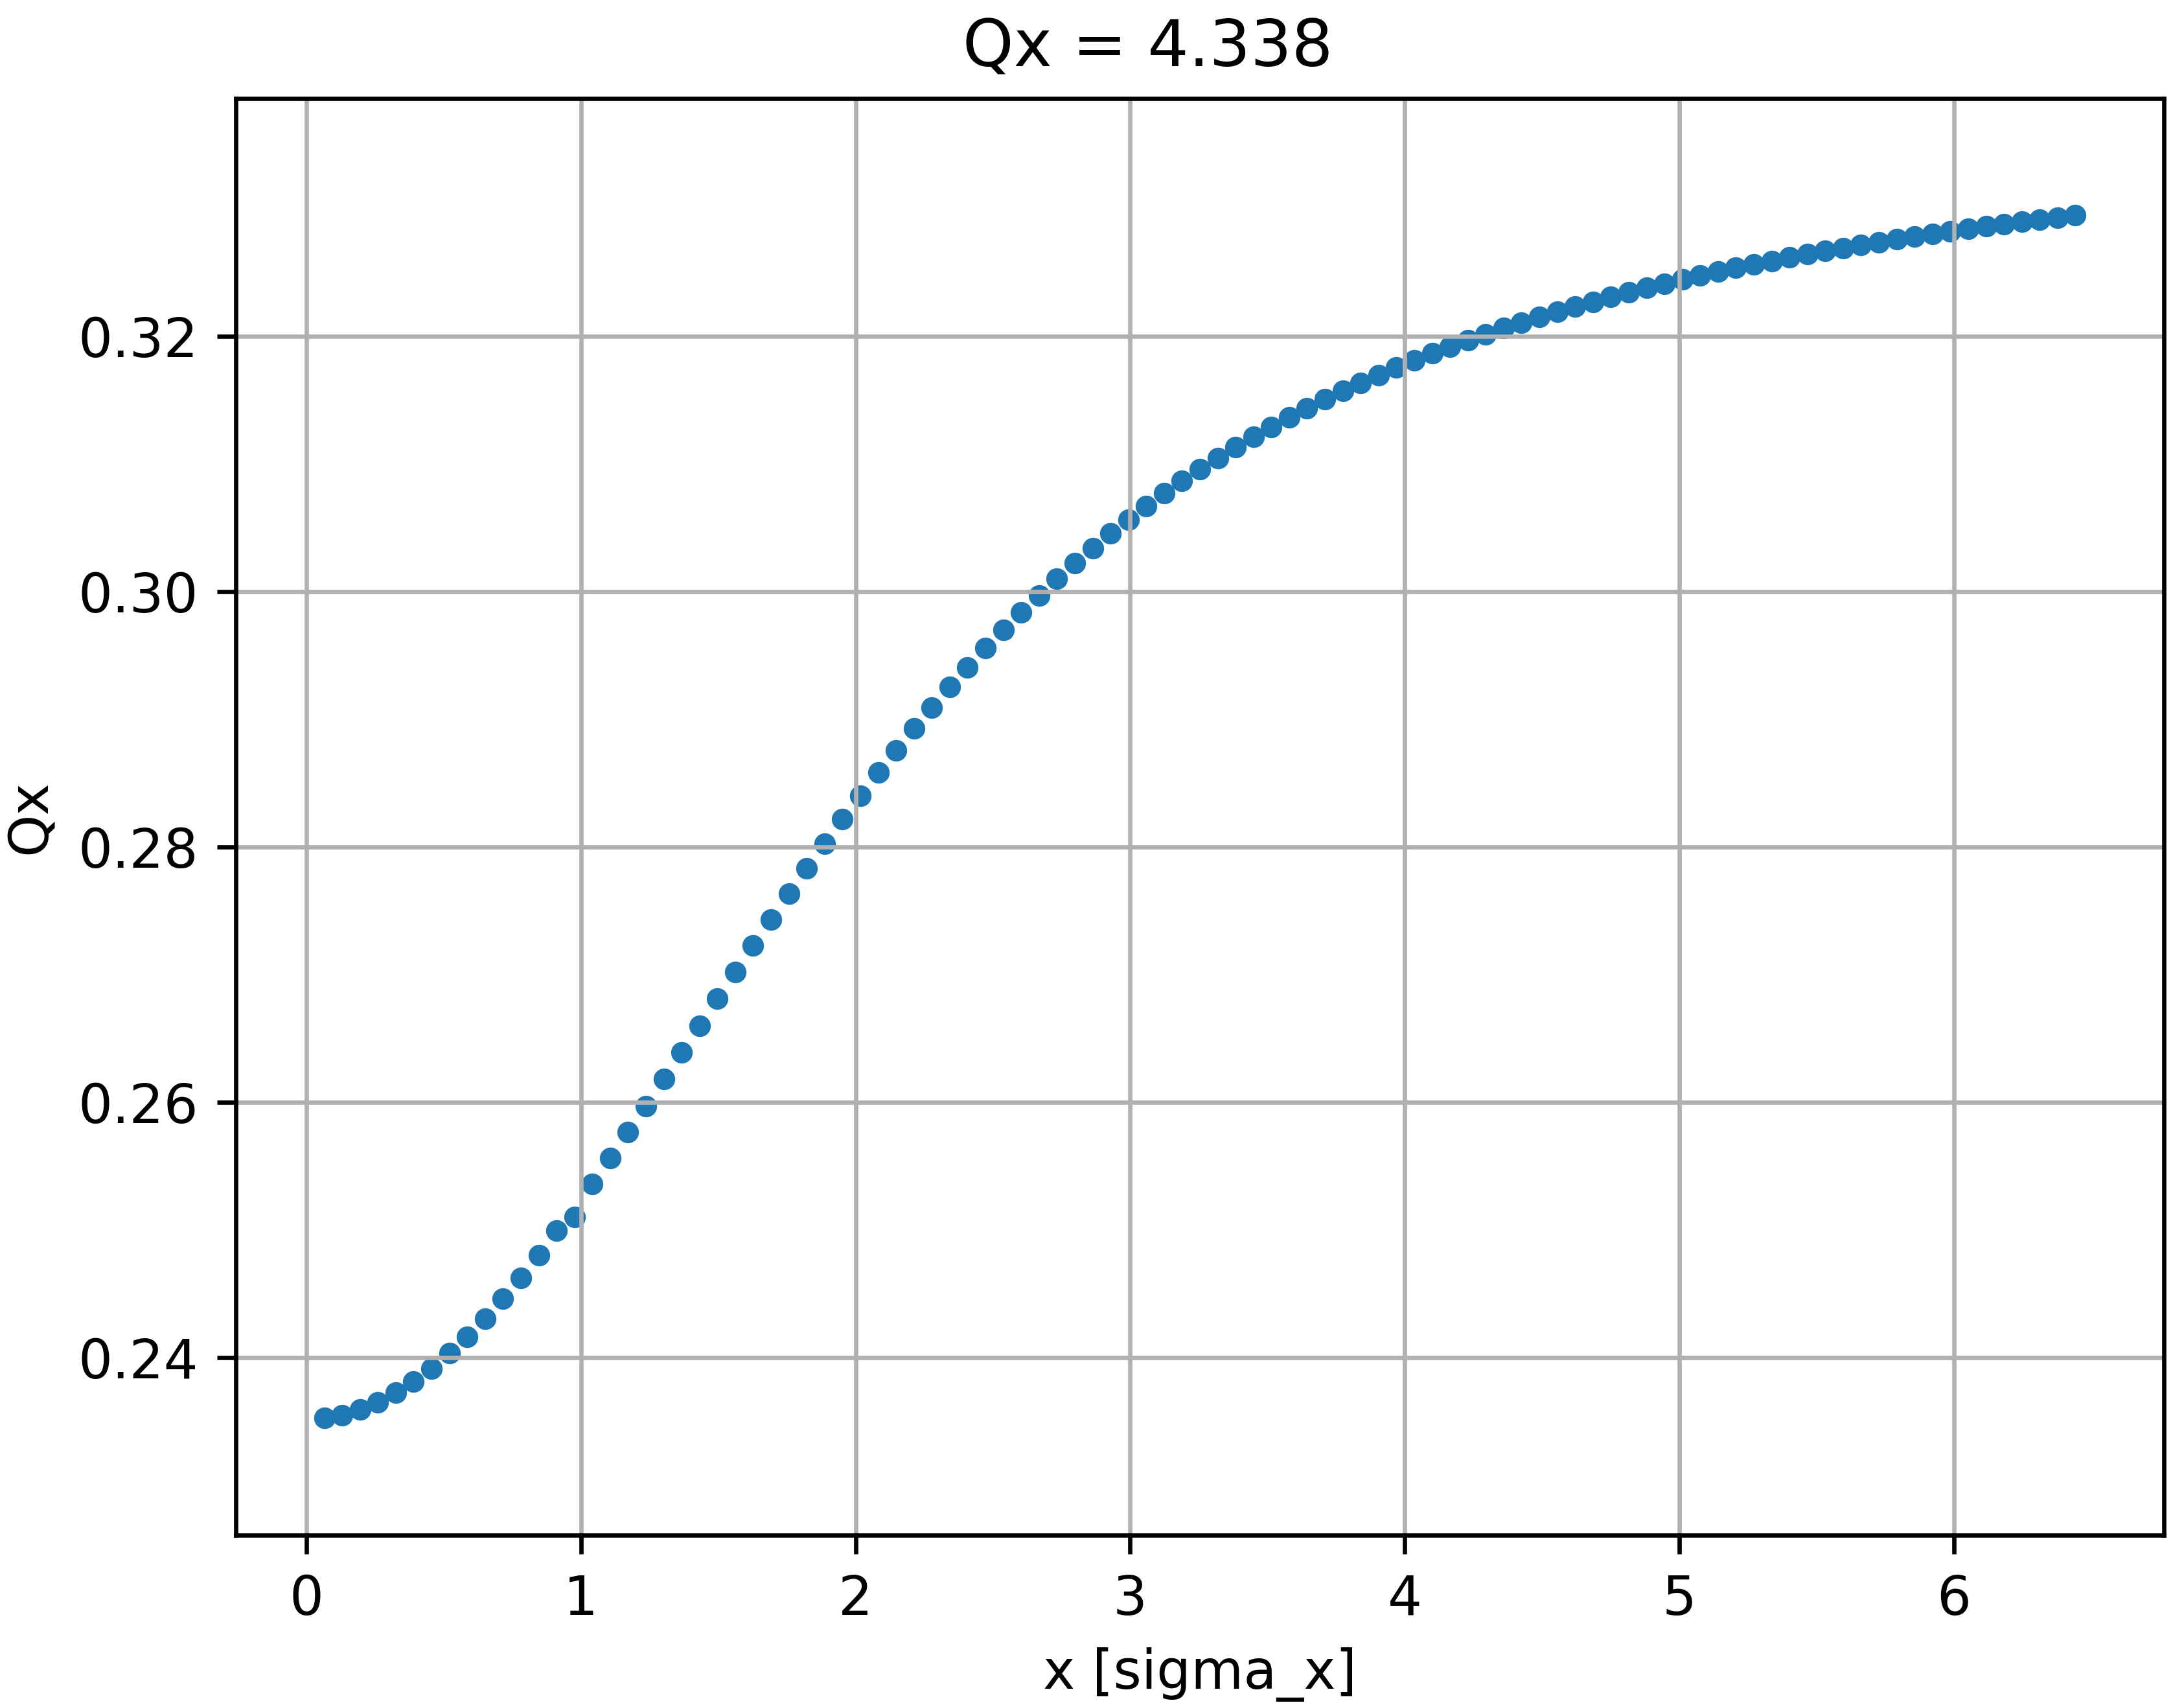
\includegraphics[width=\textwidth]{Step2_tune_x_PO.png}
          \caption{PTC-PyORBIT.}
          \label{fig:step2H_po}
        \end{subfigure}
        \caption{Step2: Horizontal tune with space charge.}
        \label{fig:step2H}
\end{figure}

\begin{figure}
        \centering
        \begin{subfigure}{.5\textwidth}
          \centering
          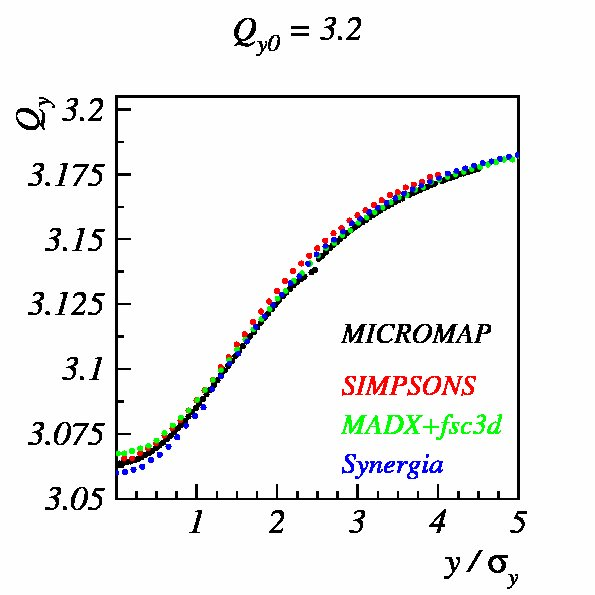
\includegraphics[width=\textwidth]{Step2_tune_y.png}
          \caption{MICROMAP and SIMPSONS.}
          \label{fig:step2V_m}
        \end{subfigure}~~~~~~
        \begin{subfigure}{.5\textwidth}
          \centering
          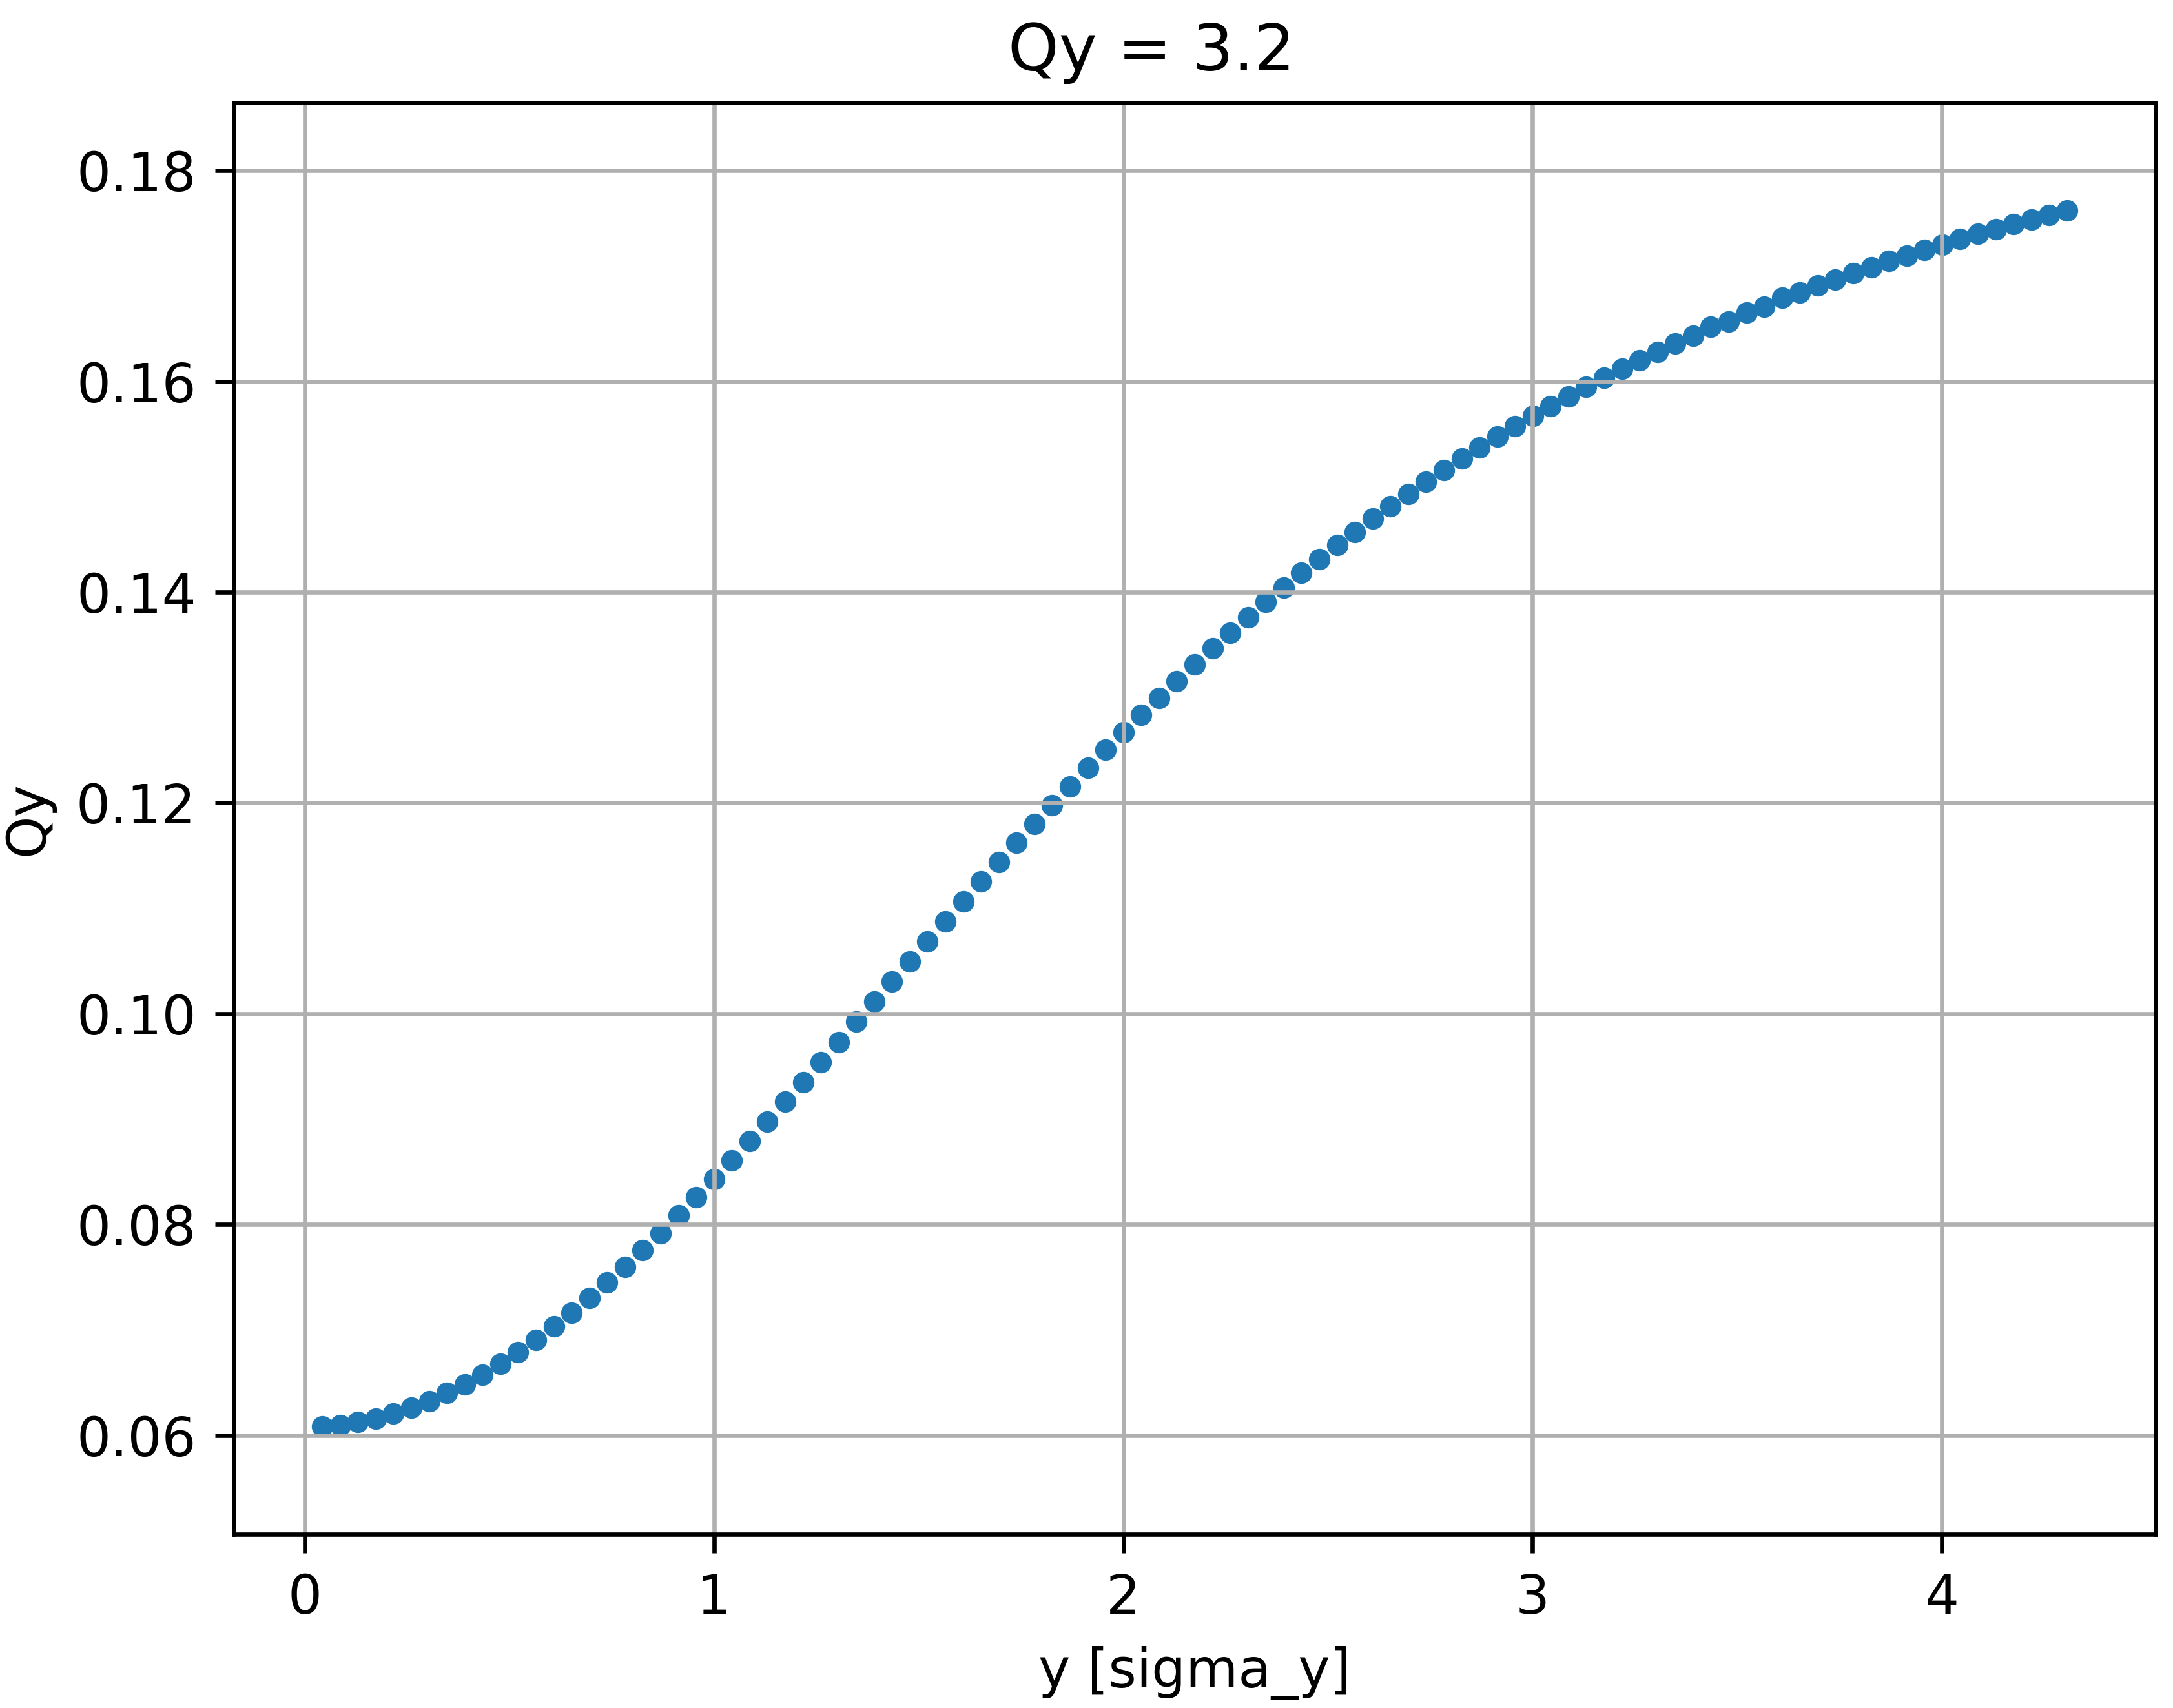
\includegraphics[width=\textwidth]{Step2_tune_y_PO.png}
          \caption{PTC-PyORBIT.}
          \label{fig:step2V_po}
        \end{subfigure}
        \caption{Step2: Vertical tune with space charge.}
        \label{fig:step2V}
\end{figure}


\section{Step 3: Tunes with sextupole on at $Q_x$ = 4.338}

The third step is to benchmark the dependence of a test particle tune from its amplitude when the sextupole is on. The calculation of the tune is performed as described in step 2. In order to visualize the island not too far from the bunch center we take the tunes: $Q_x$ = 4.338, $Q_y$ = 3.2. Note that the island is not visible because we are too far with respect to the range explored: in order to see the island we need to take a tune further from the resonance, this is done in the next step. The particle amplitudes are as defined in Step 2. 

\begin{figure}
        \centering
        \begin{subfigure}{.5\textwidth}
          \centering
          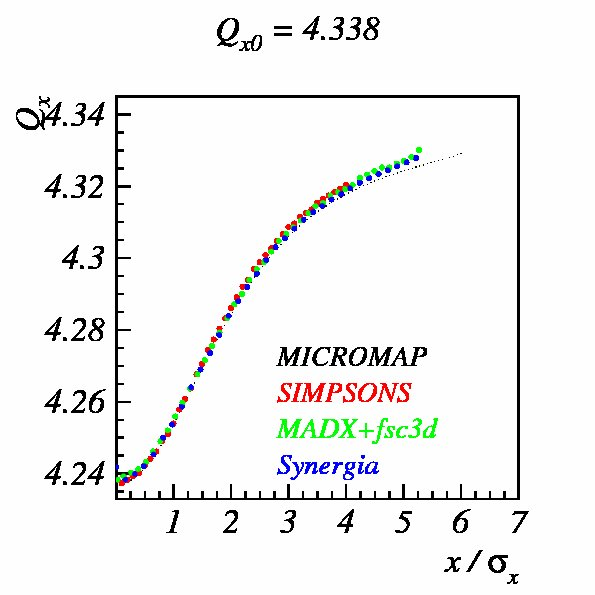
\includegraphics[width=\textwidth]{Step3_tune_x.png}
          \caption{MICROMAP and SIMPSONS.}
          \label{fig:step3H_m}
        \end{subfigure}~~~~~~
        \begin{subfigure}{.5\textwidth}
          \centering
          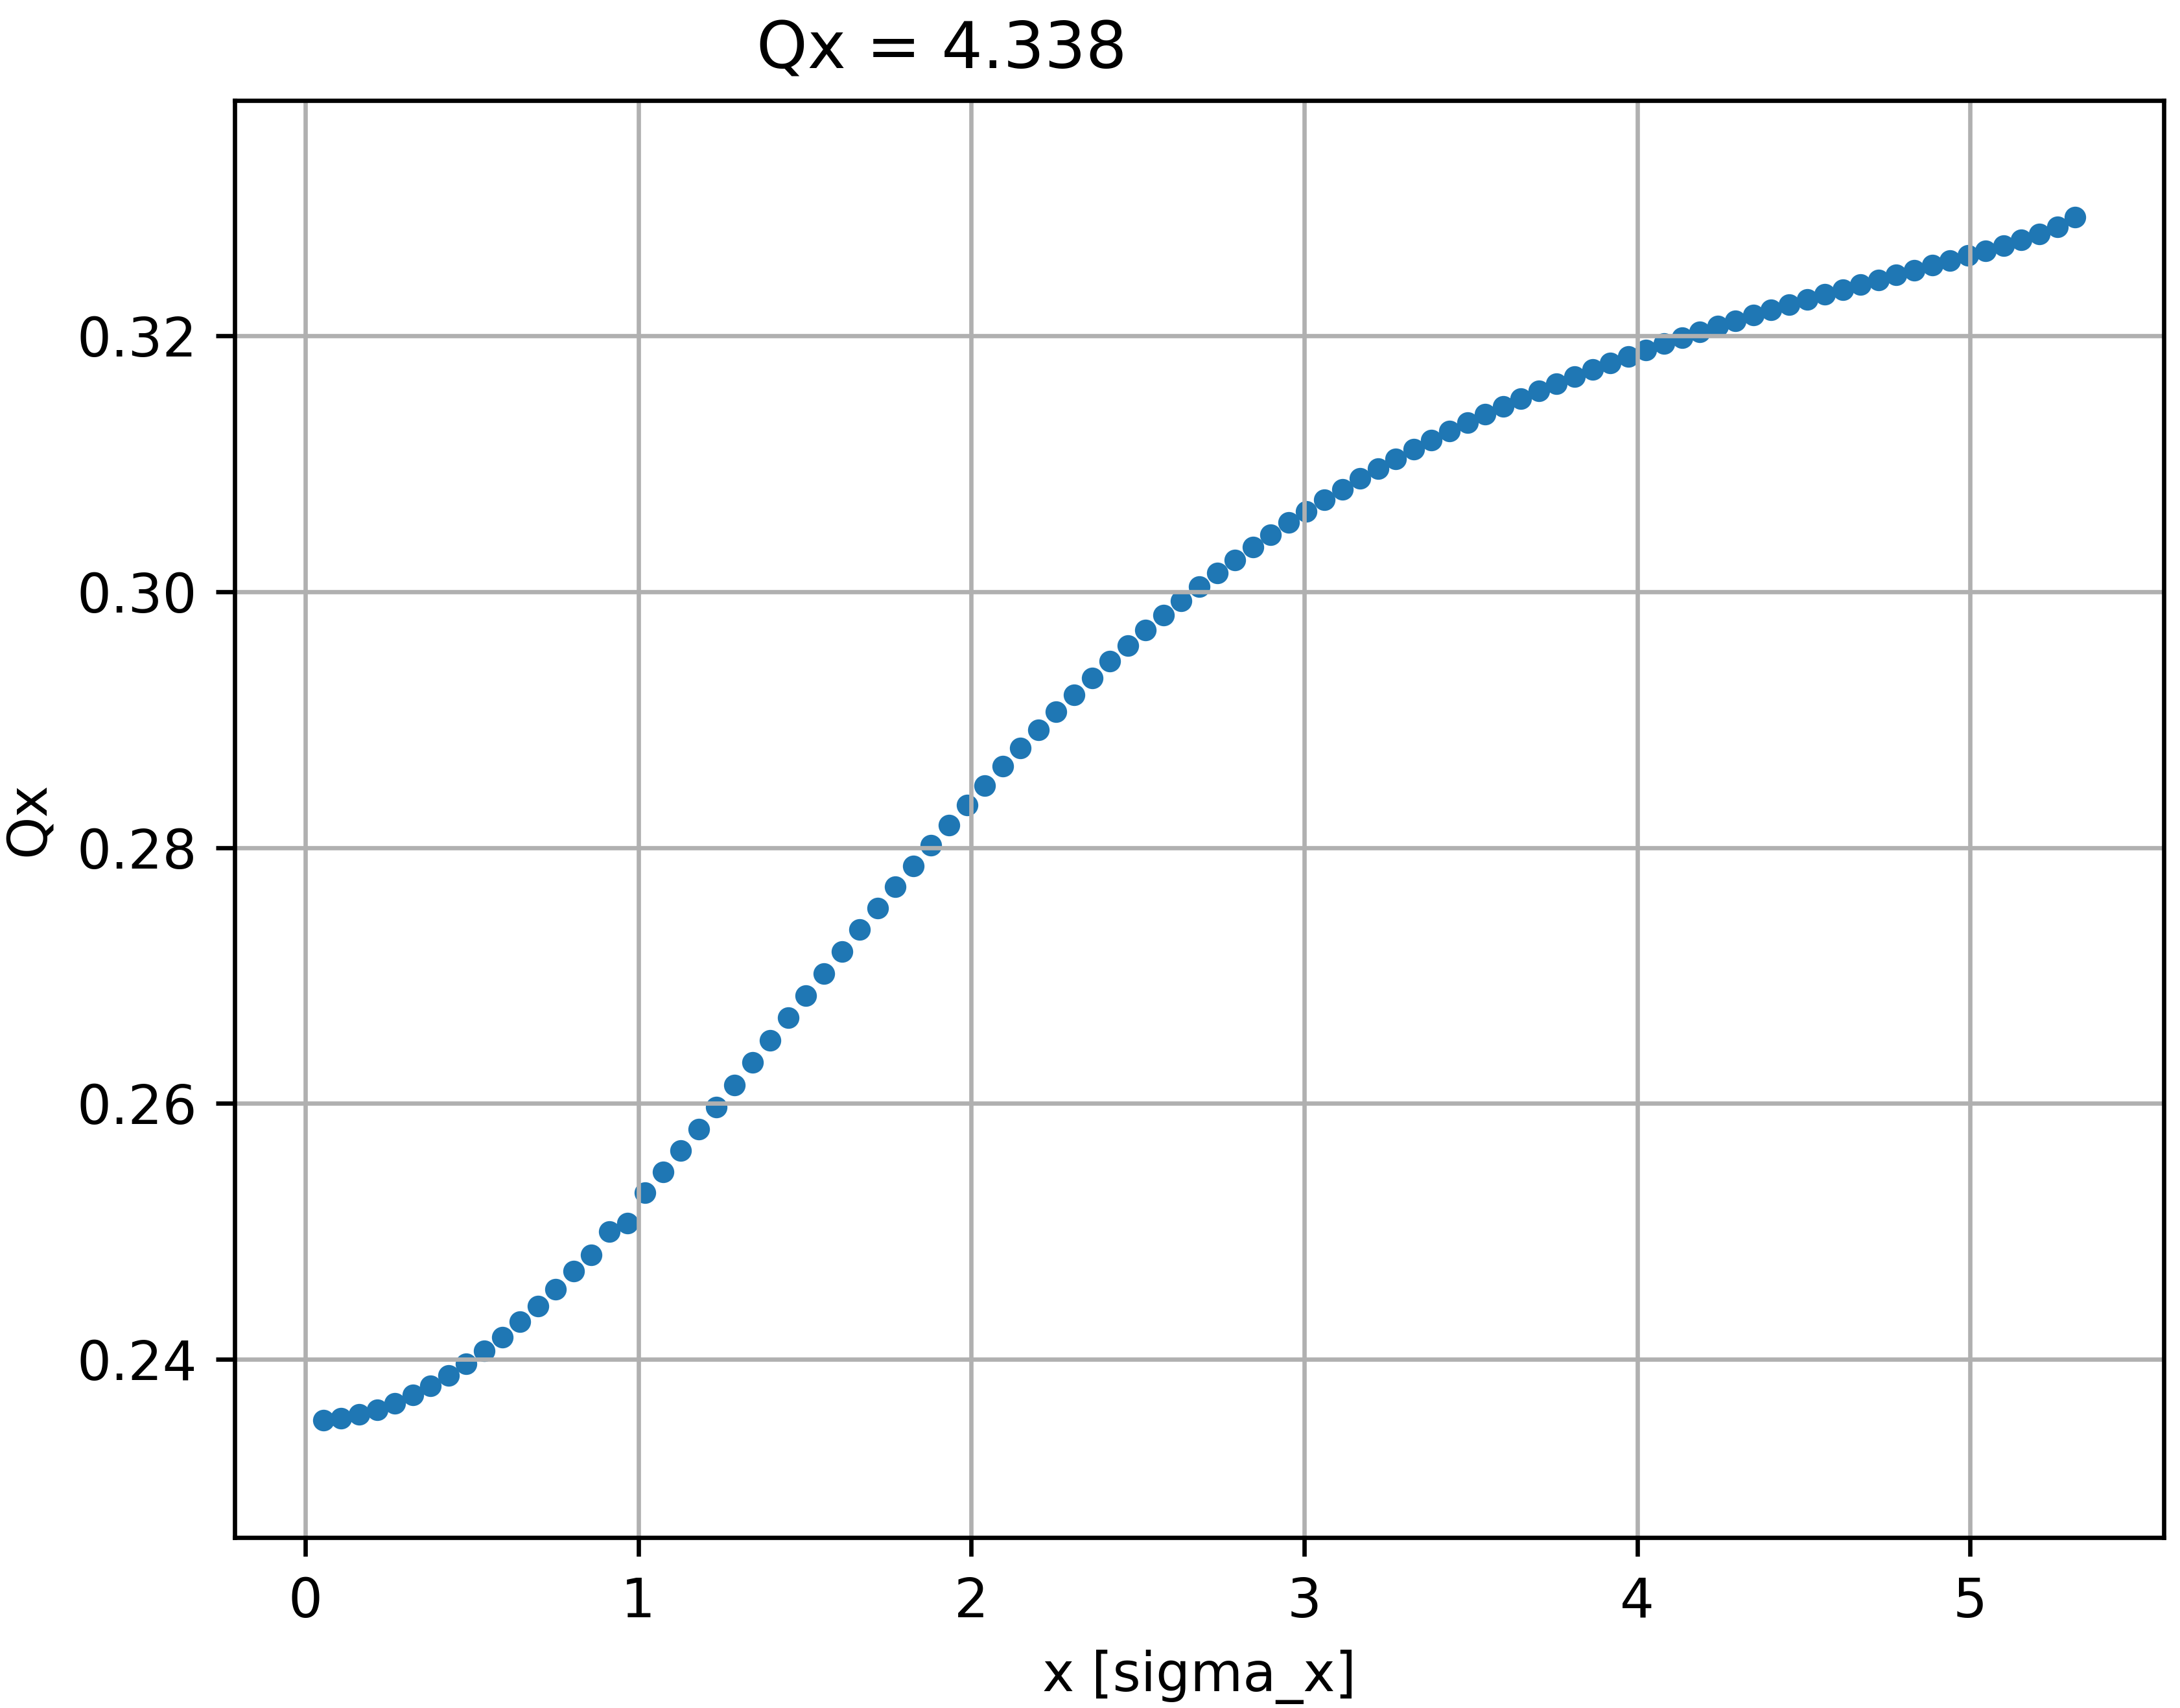
\includegraphics[width=\textwidth]{Step3_tune_x_PO.png}
          \caption{PTC-PyORBIT.}
          \label{fig:step3H_po}
        \end{subfigure}
        \caption{Step3: Horizontal tune with space charge and Sextupole.}
        \label{fig:step3H}
\end{figure}

\begin{figure}
        \centering
        \begin{subfigure}{.5\textwidth}
          \centering
          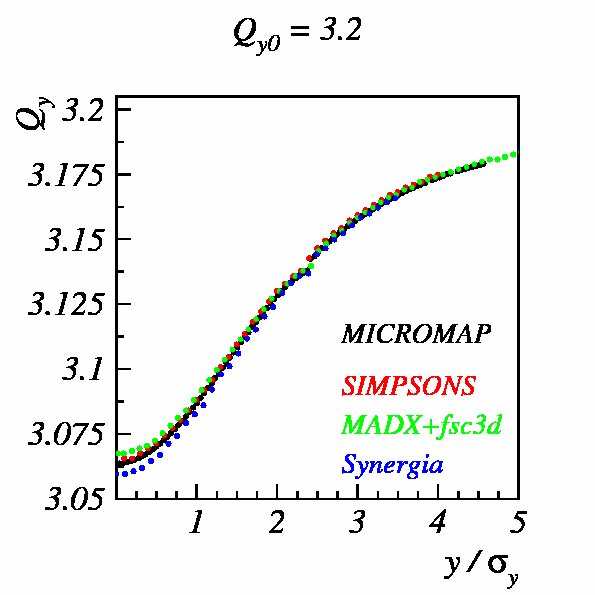
\includegraphics[width=\textwidth]{Step3_tune_y.png}
          \caption{MICROMAP and SIMPSONS.}
          \label{fig:step3V_m}
        \end{subfigure}~~~~~~
        \begin{subfigure}{.5\textwidth}
          \centering
          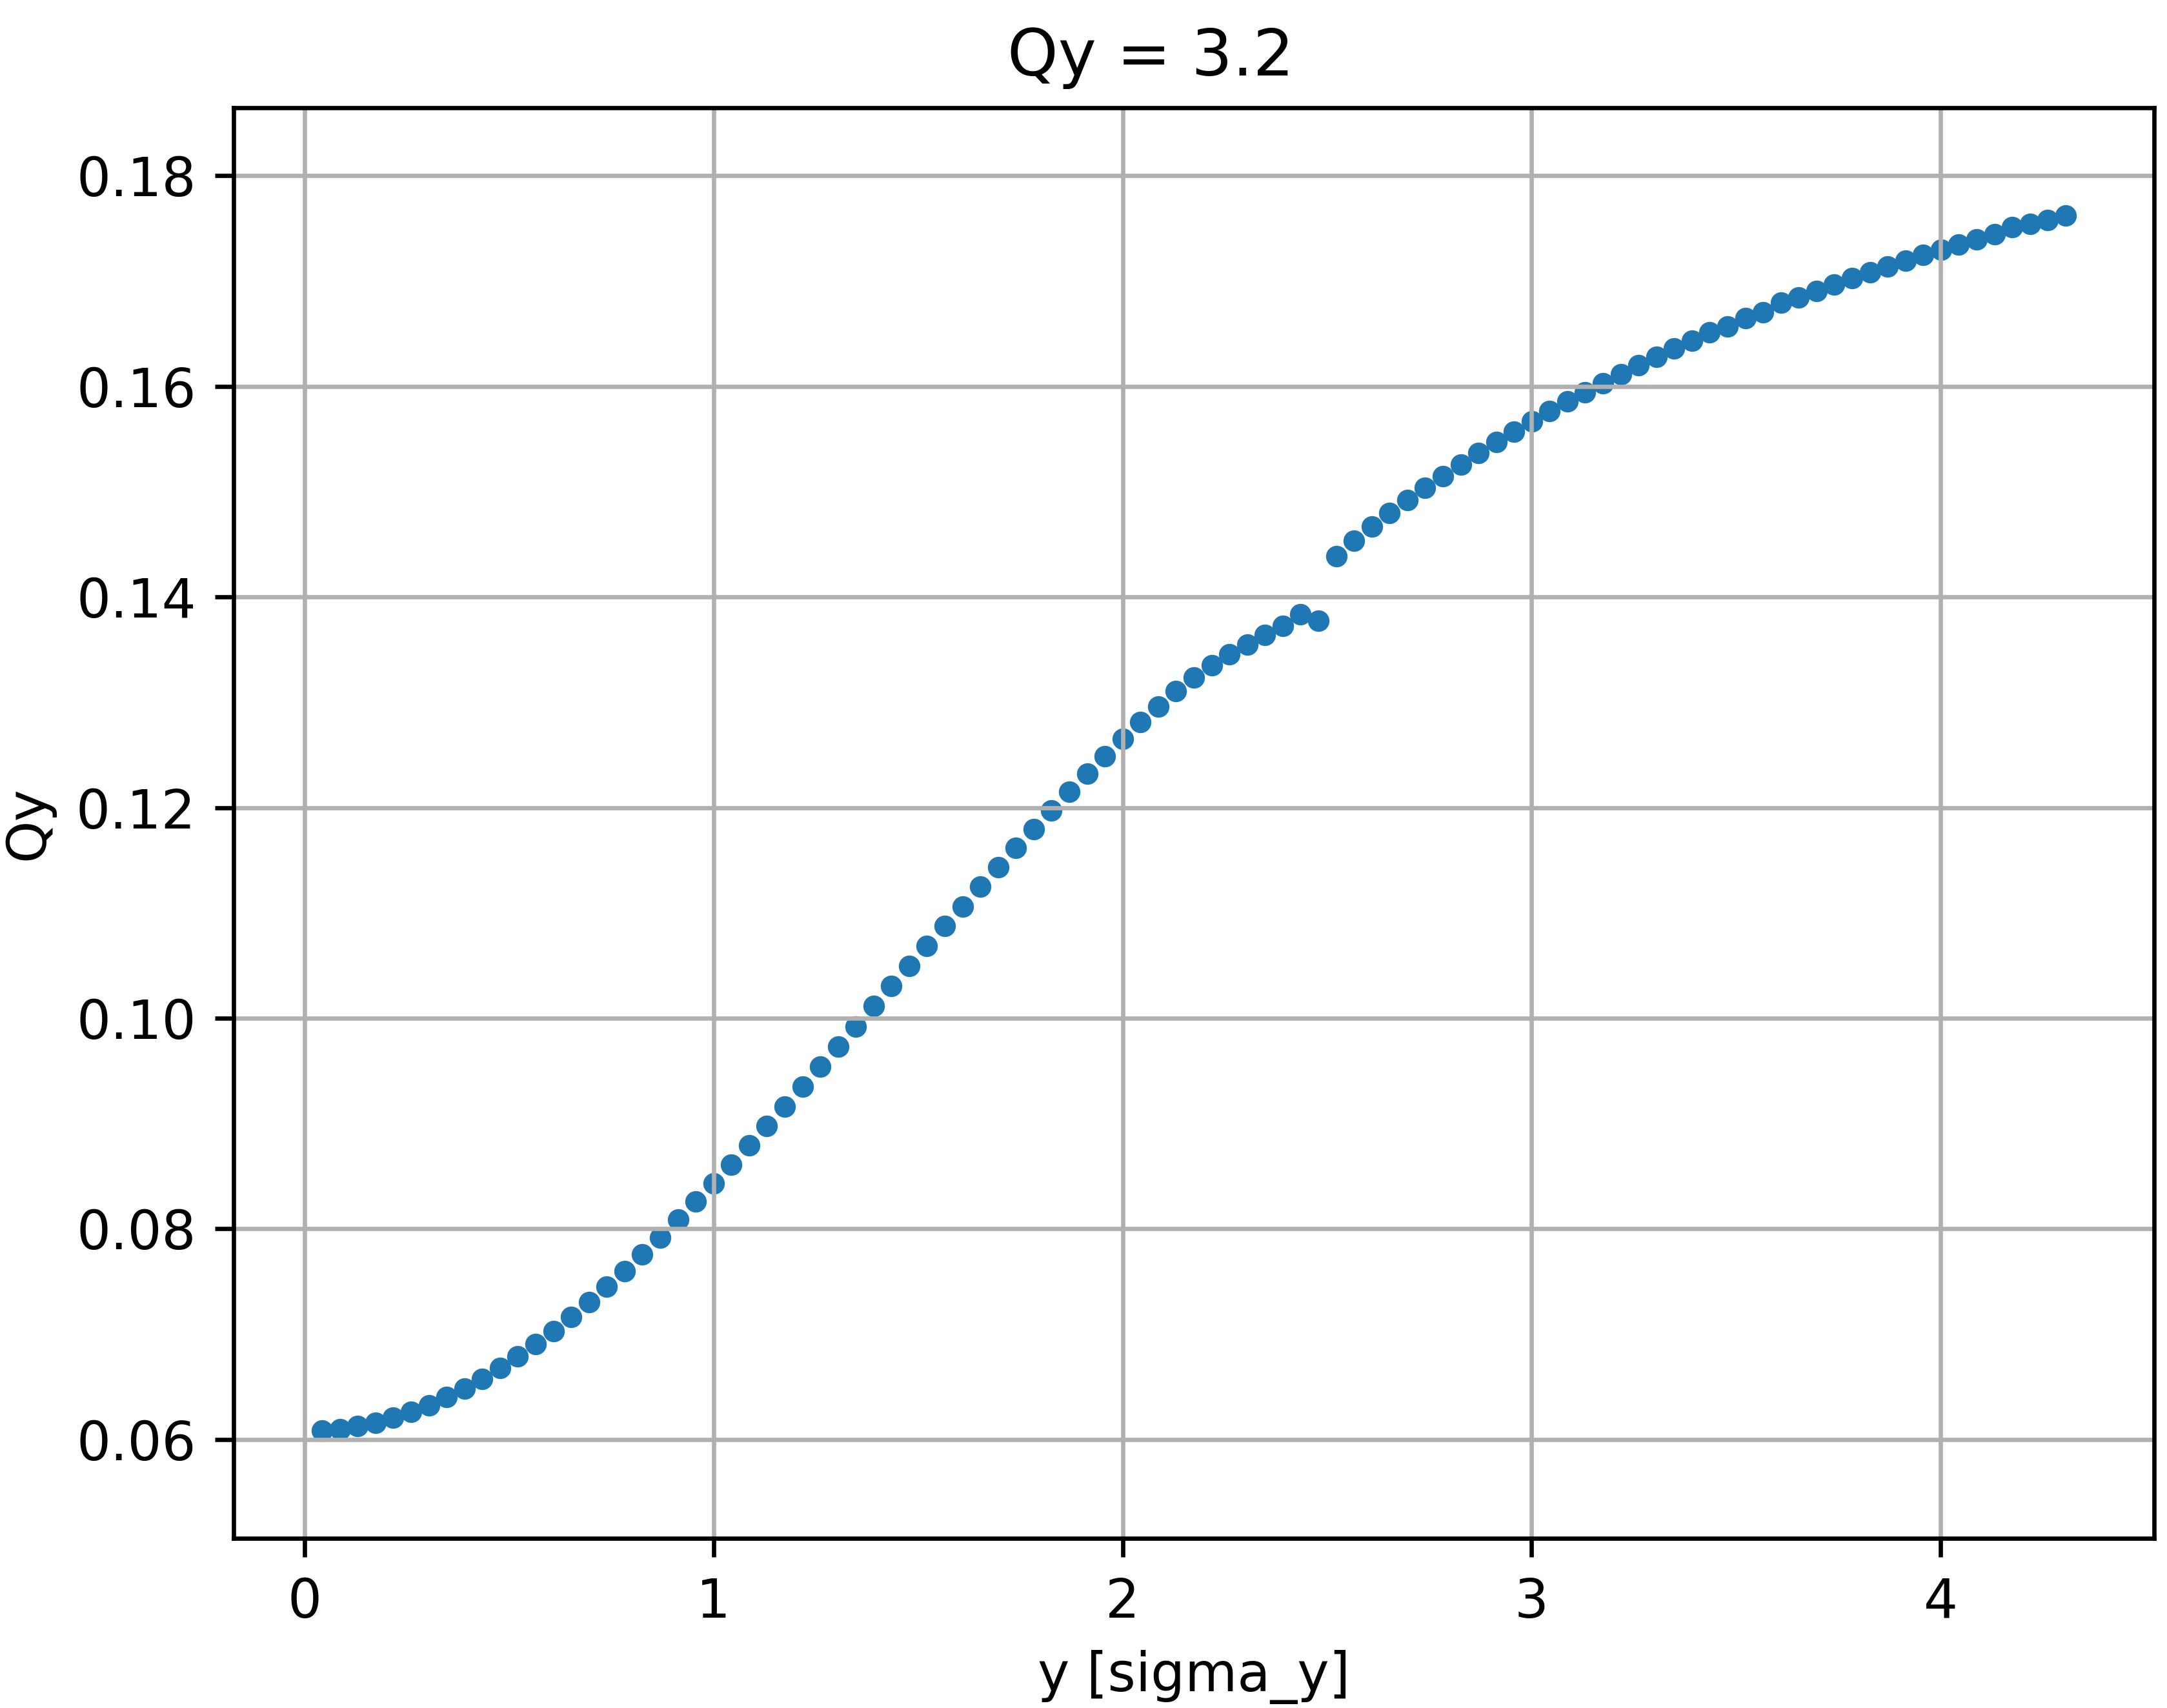
\includegraphics[width=\textwidth]{Step3_tune_y_PO.png}
          \caption{PTC-PyORBIT.}
          \label{fig:step3V_po}
        \end{subfigure}
        \caption{Step3: Vertical tune with space charge and Sextupole.}
        \label{fig:step3V}
\end{figure}

\section{Step 4: Tunes with sextupole on at $Q_x$ = 4.3504}

The fourth step is to benchmark the dependence of a test particle tune from its amplitude when the sextupole is on. The calculation of the tune is performed as described in step. In order to visualize the island far from the bunch center we now take the tunes closer to the 3rd order resonance i.e.: $Q_x$ = 4.3504, $Q_y$ = 3.2.

\begin{figure}
        \centering
        \begin{subfigure}{.5\textwidth}
          \centering
          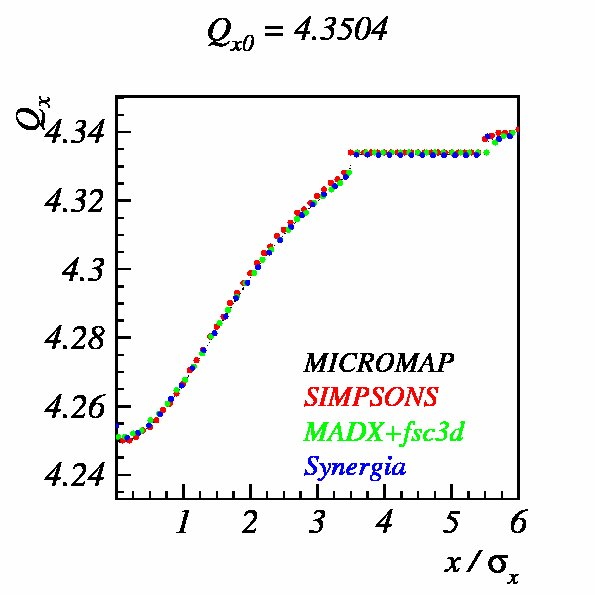
\includegraphics[width=\textwidth]{Step4_tune_x.png}
          \caption{MICROMAP and SIMPSONS.}
          \label{fig:step4H_m}
        \end{subfigure}~~~~~~
        \begin{subfigure}{.5\textwidth}
          \centering
          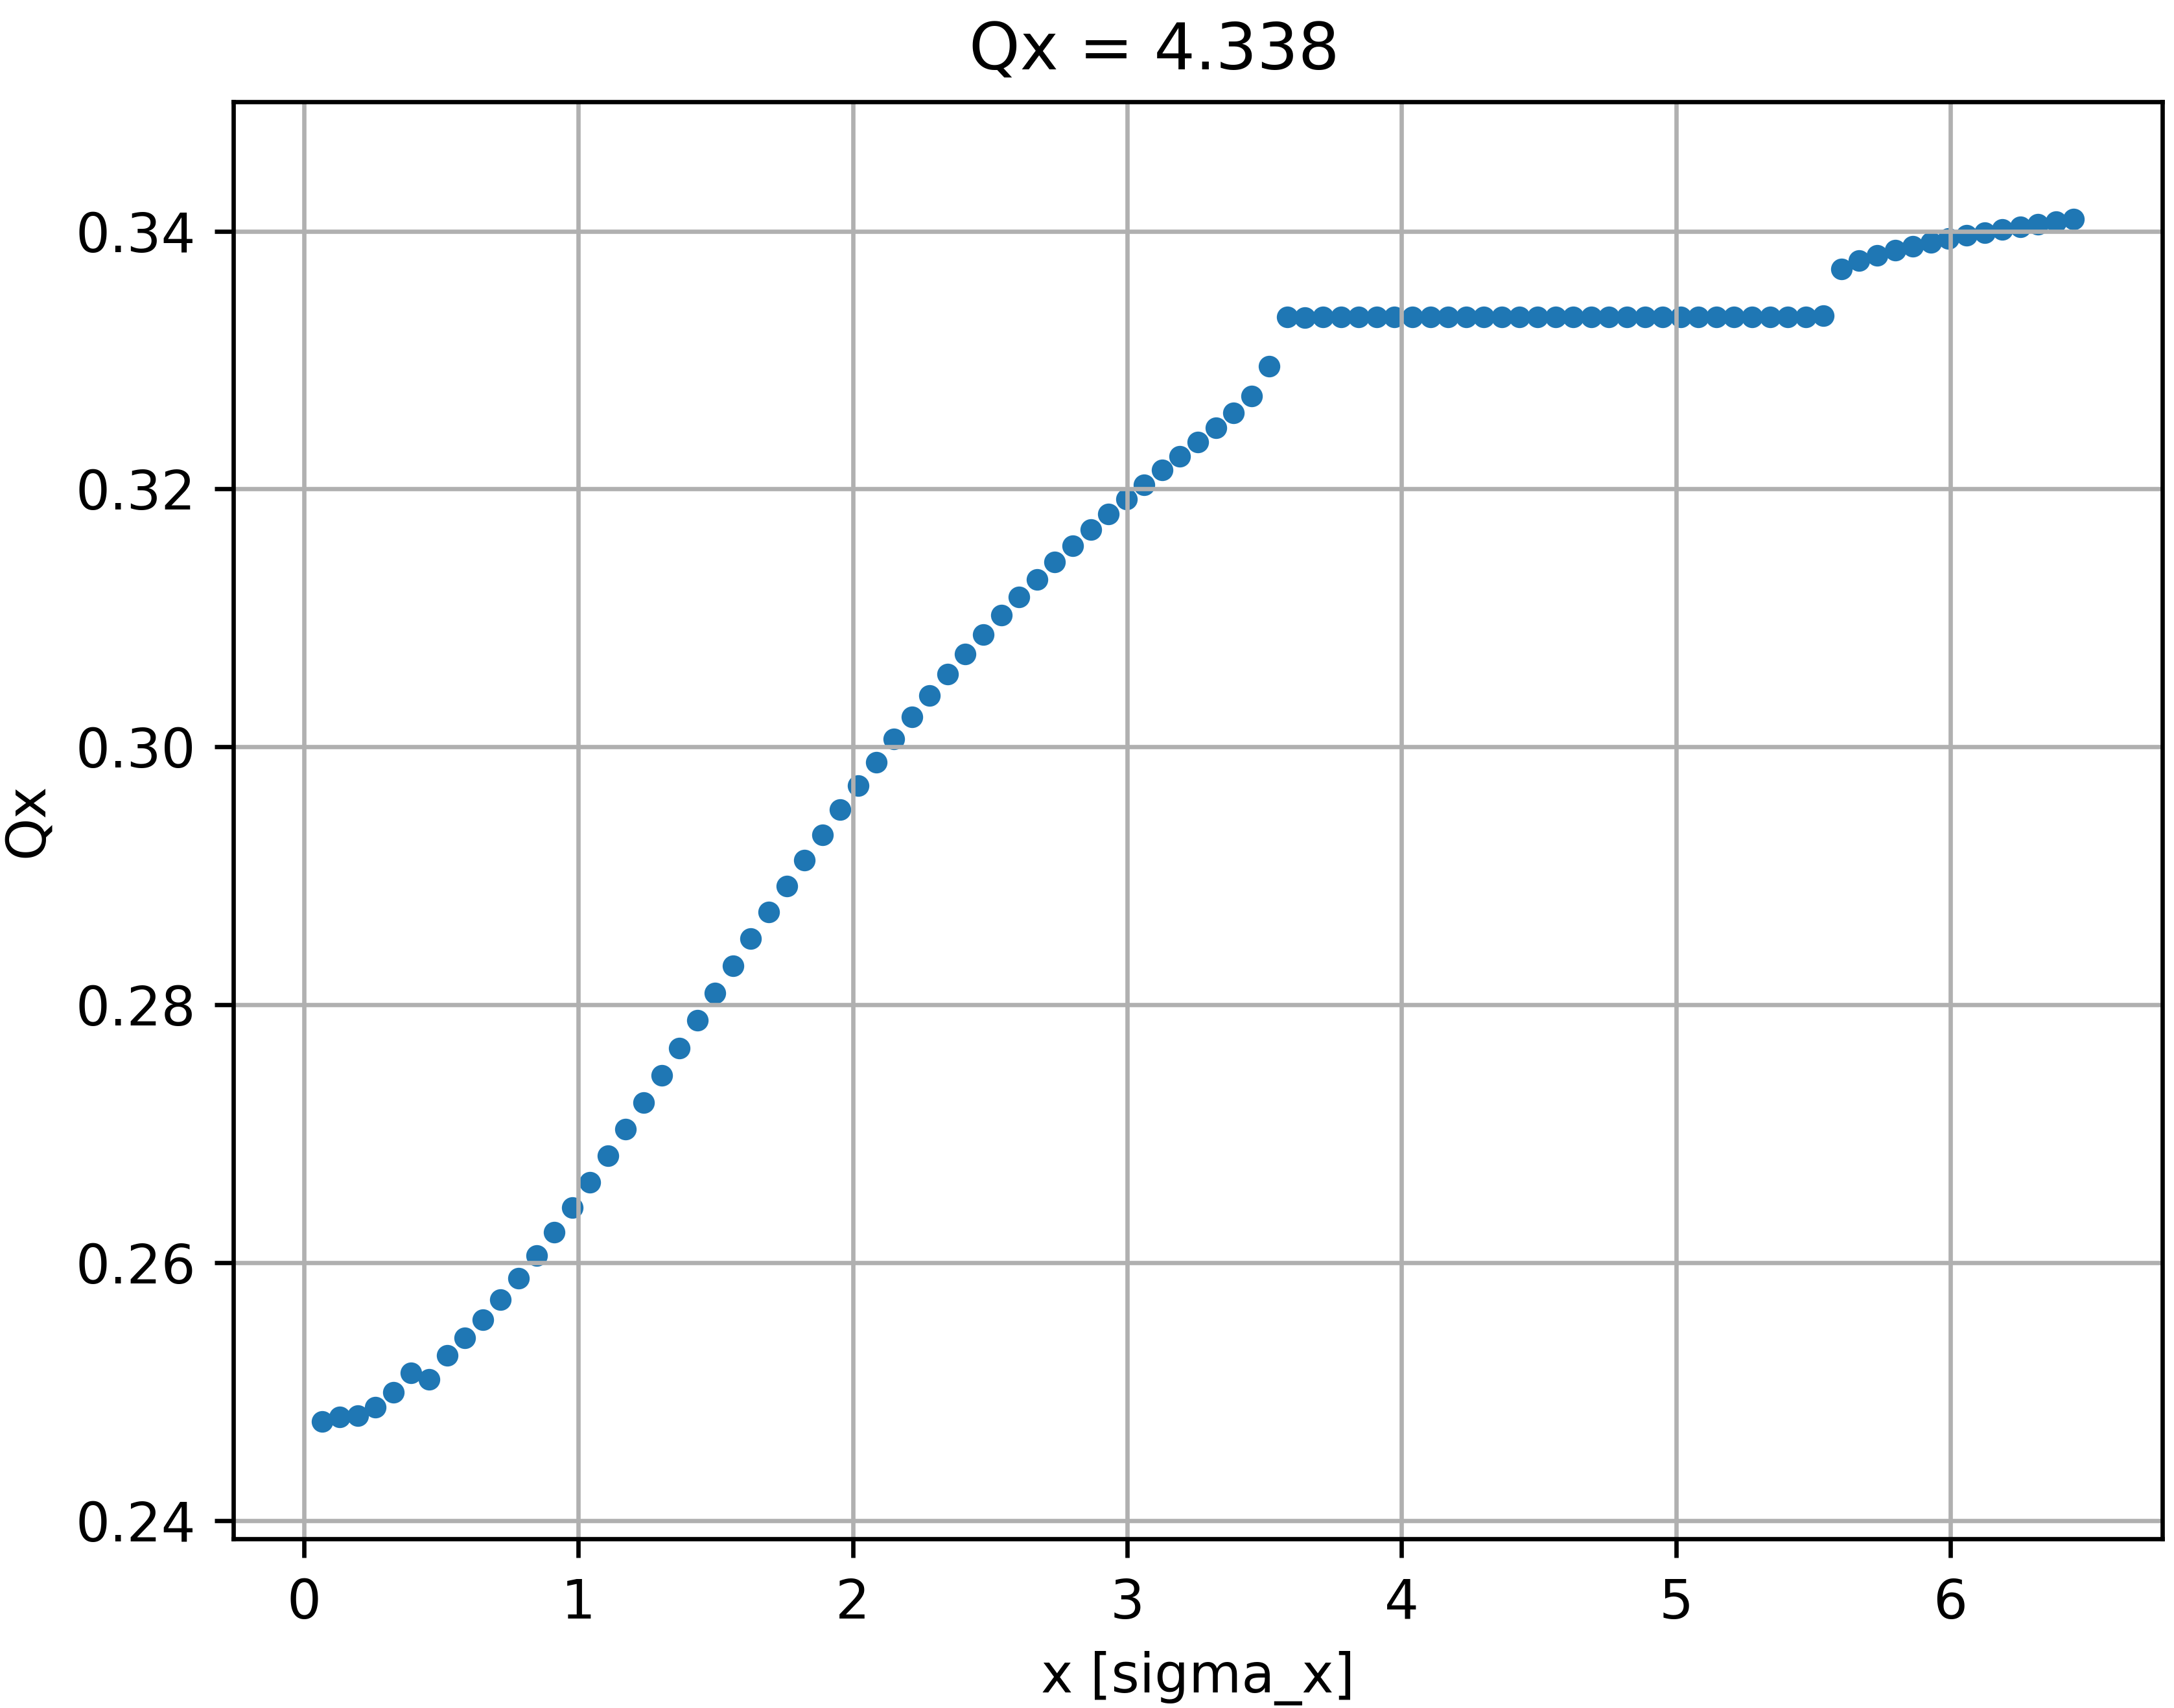
\includegraphics[width=\textwidth]{Step4_tune_x_PO.png}
          \caption{PTC-PyORBIT.}
          \label{fig:step4H_po}
        \end{subfigure}
        \caption{Step4: Horizontal tune with space charge and Sextupole at $Q_x$ = 4.3504.}
        \label{fig:step4H}
\end{figure}

\begin{figure}
        \centering
        \begin{subfigure}{.5\textwidth}
          \centering
          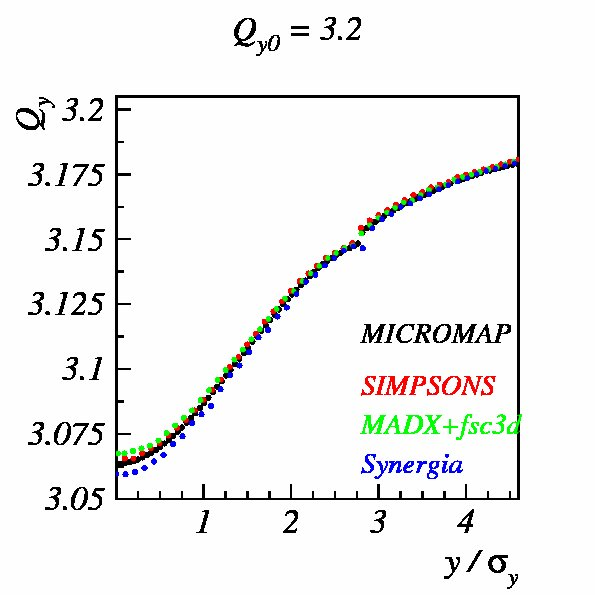
\includegraphics[width=\textwidth]{Step4_tune_y.png}
          \caption{MICROMAP and SIMPSONS.}
          \label{fig:step4V_m}
        \end{subfigure}~~~~~~
        \begin{subfigure}{.5\textwidth}
          \centering
          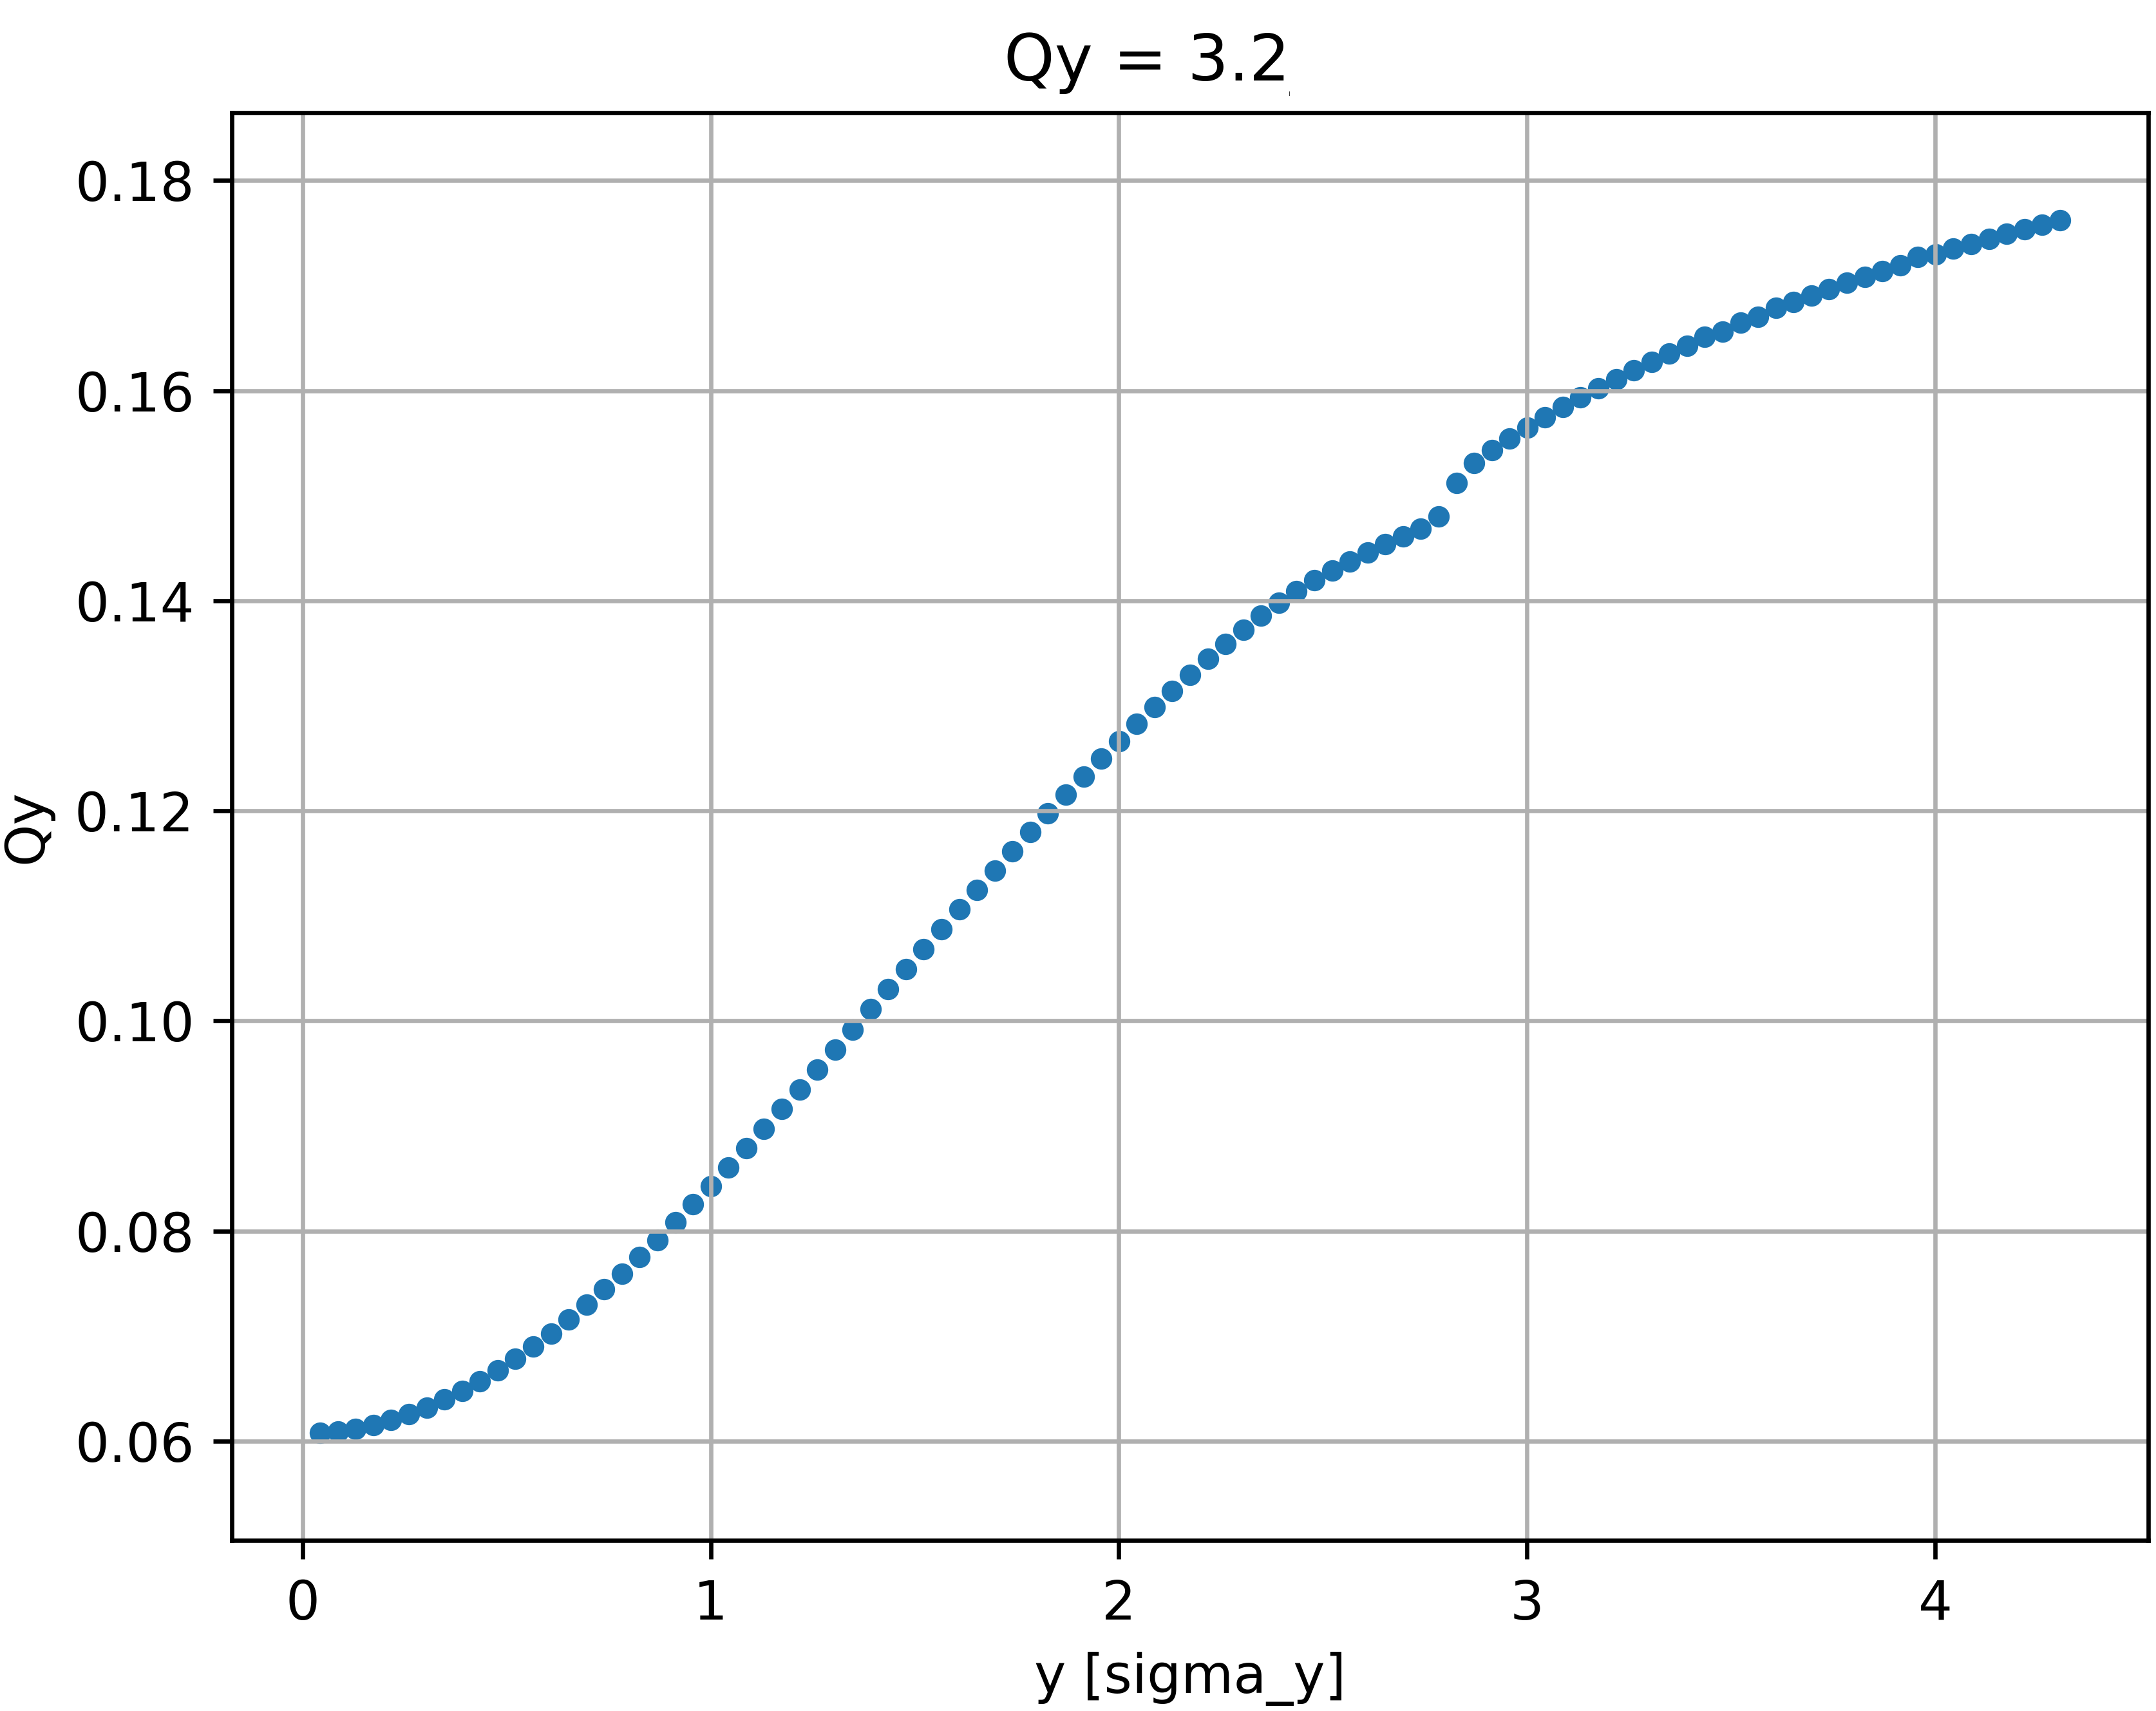
\includegraphics[width=\textwidth]{Step4_tune_y_PO.png}
          \caption{PTC-PyORBIT.}
          \label{fig:step4V_po}
        \end{subfigure}
        \caption{Step4: Vertical tune with space charge and Sextupole.}
        \label{fig:step4V}
\end{figure}

\section{Step 5: Phase space with space charge and sextupole on at $Q_x$ = 4.3504}

The fifth step is to benchmark the phase space with test particles when the sextupole is on and in the presence of space charge. Here the orbits are already subjected to trapping as the synchrotron motion is not frozen.

\begin{figure}
        \centering
        \begin{subfigure}{.5\textwidth}
          \centering
          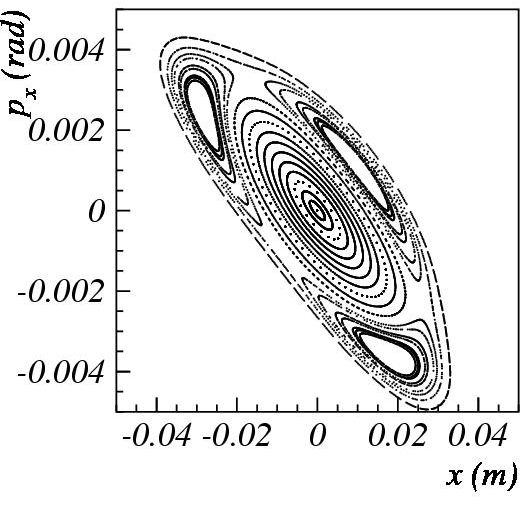
\includegraphics[width=\textwidth]{Step5_phase-space.png}
          \caption{MICROMAP and SIMPSONS.}
          \label{fig:step5_m}
        \end{subfigure}~~~~~~
        \begin{subfigure}{.5\textwidth}
          \centering
          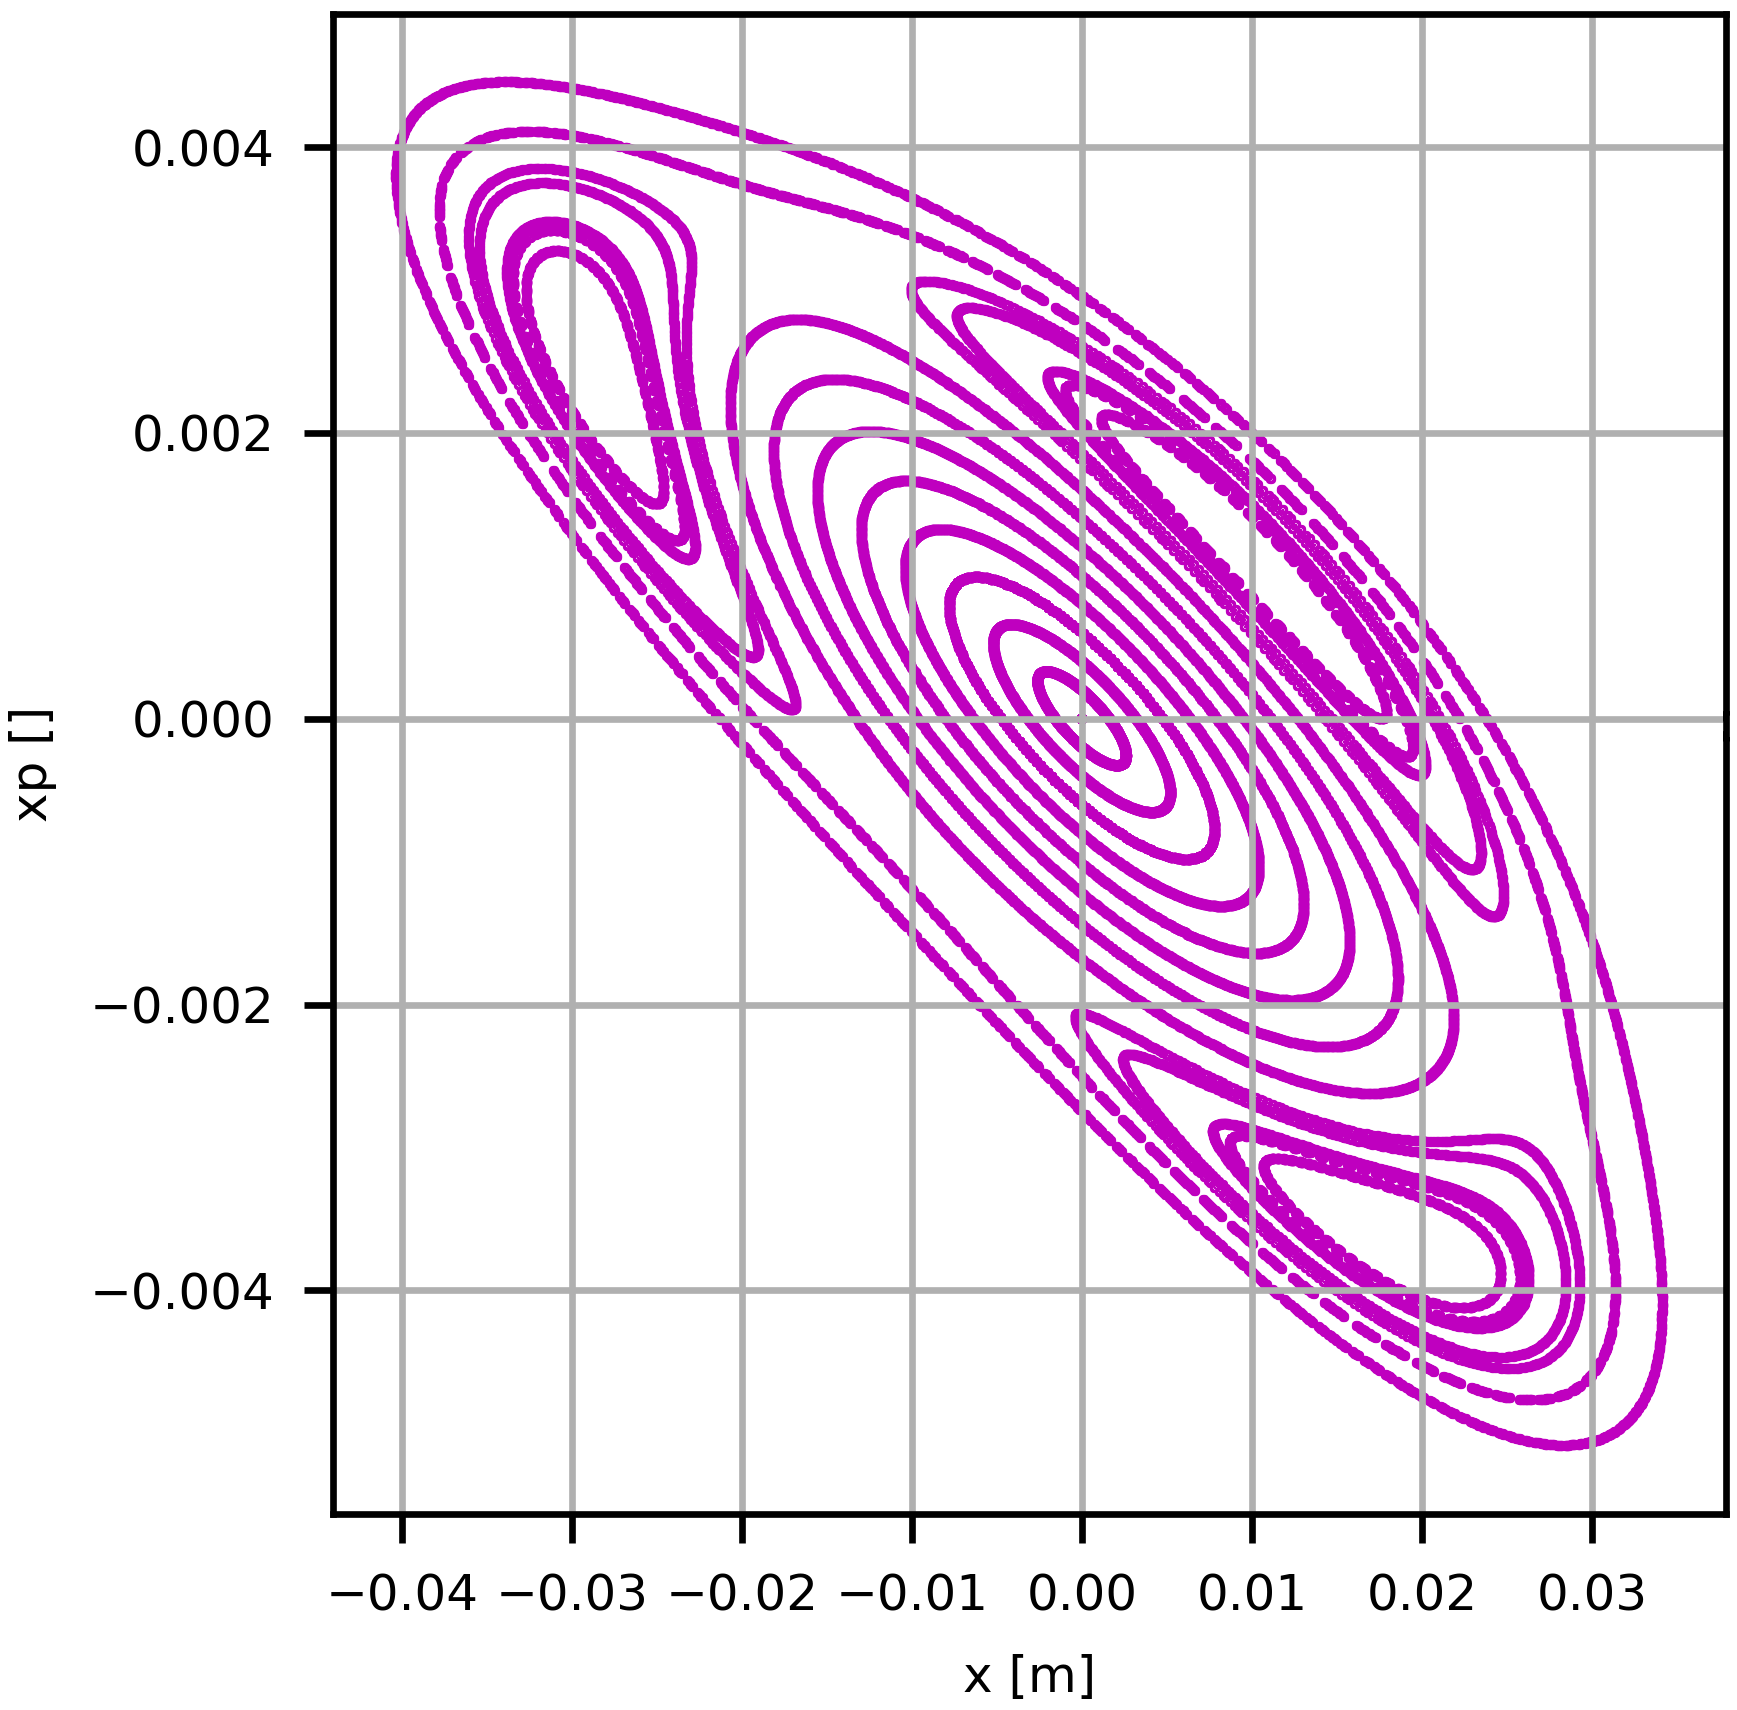
\includegraphics[width=\textwidth]{Step5_phase-space_PO.png}
          \caption{PTC-PyORBIT.}
          \label{fig:step1_po}
        \end{subfigure}
        \caption{Step5: Phase space with sextupole and space charge at $Q_x$ = 4.3504.}
        \label{fig:step1}
\end{figure}


\section{Step 6: Benchmarking of trapping in 1 synchrotron oscillation for $Q_s$ = 1/15000}

The sixth step is to benchmark the trapping of 1 test particle during 1 synchrotron oscillation. The parameters used are those of the steps 4 and 5. In order to visualize the increase of the single particle invariant we take the tunes: $Q_x$ = 4.3504, $Q_y$ = 3.2.

The test particle has the following initial coordinates:$x$ = 5 mm, $px = y = py = 0$ and $z = 2.5 \sigma_z$, $pz$ = 0.

Note that the probability of trapping is very sensitive to initial conditions. Therefore it may happen that "scattering" is seen in place of trapping. A slight variation of the particle initial coordinates should allow the trapping phenomena as in Fig~\ref{fig:step6}.

One synchrotron oscillation takes 15000 turns. We compare the trapping by plotting the evolution of the single particle emittance $\epsilon_x = \beta_x px^2 + 2 \alpha_x x px + \gamma_x x^2$ of the test particle (normalised with the initial value) vs. number of turns. Note that the maximum amplitude of the center island is roughly 30 mm (see step 5), and a particle with initial coordinates $x$ = 5 mm $px$ = 0 has maximum amplitude of 8.125 mm. Therefore one expects a maximum emittance growth of $\frac{\epsilon_x}{\epsilon_{x0}} \approx \left( \frac{30}{8.125}\right)^2$ = 13.6.

The synchrotron motion in PTC-PyORBIT is performed as an energy kick $dE = dE_0 + z F$ where $F$ is the restoring force required to maintain a synchrotron period of 15000 turns, performed once per turn.

\begin{figure}[!htb]
        \centering
        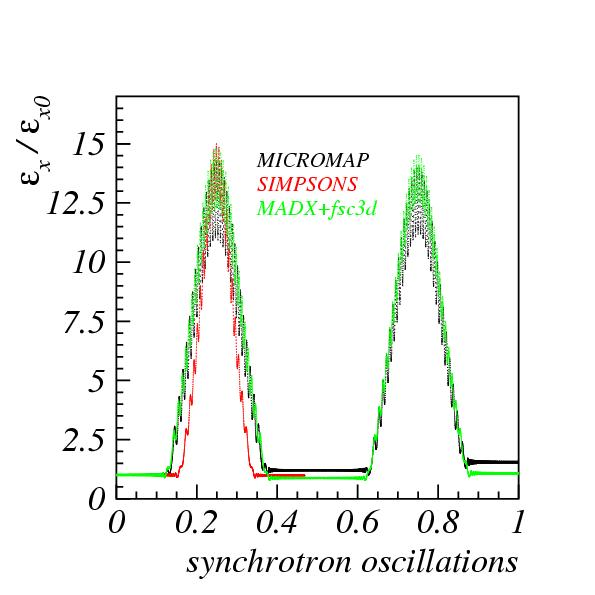
\includegraphics[width=0.5\columnwidth]{Step6_trapping.jpg}
        \caption{Step6.}
        \label{fig:step6}
\end{figure}

\section{Step 7: Benchmarking of trapping in 1 synchrotron oscillation for $Q_s$ = 1/1000}

First we find the linear restoring force required to maintain a synchrotron tune of $Q_s = \frac{1}{1000}$ without the sextupole, and without space charge. Using an iterative approach, with the suggested reference particle ($x$ = 5 mm, $px = y = py = 0$ and $z = 2.5 \sigma_z$, $pz$ = 0) the force required was found to be $F = -4.4038 \cdot 10^{-9}$. The poincar\'{e} section is shown in Fig. 

\begin{figure}[!htb]
        \centering
        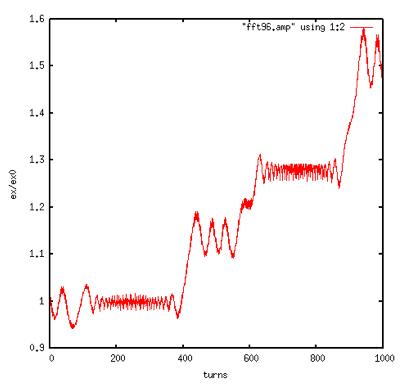
\includegraphics[width=0.5\columnwidth]{Step7_trapping_MICROMAP.jpg}
        \caption{Step7.}
        \label{fig:step7_m}
\end{figure}

\begin{figure}[!htb]
        \centering
        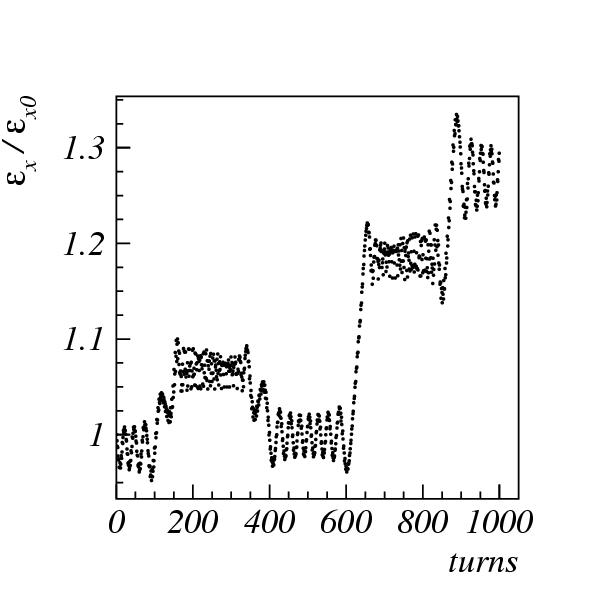
\includegraphics[width=0.5\columnwidth]{Step7_trapping_SIMPSONS.jpg}
        \caption{Step7.}
        \label{fig:step7_s}
\end{figure}

\section{Step 8: Benchmarking of trapping in $5 \cdot 10^5$ turns for $Q_s$ = 1/1000}

\begin{figure}[!htb]
        \centering
        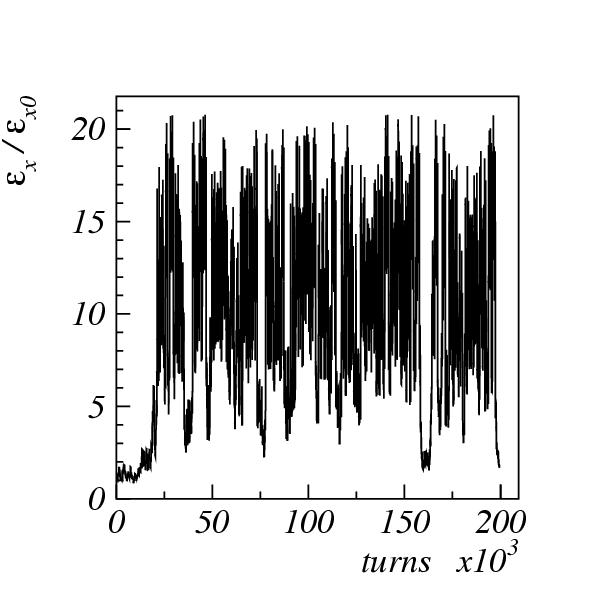
\includegraphics[width=0.5\columnwidth]{Step8_trapping_MICROMAP.jpg}
        \caption{Step8.}
        \label{fig:step8_m}
\end{figure}

\begin{figure}[!htb]
        \centering
        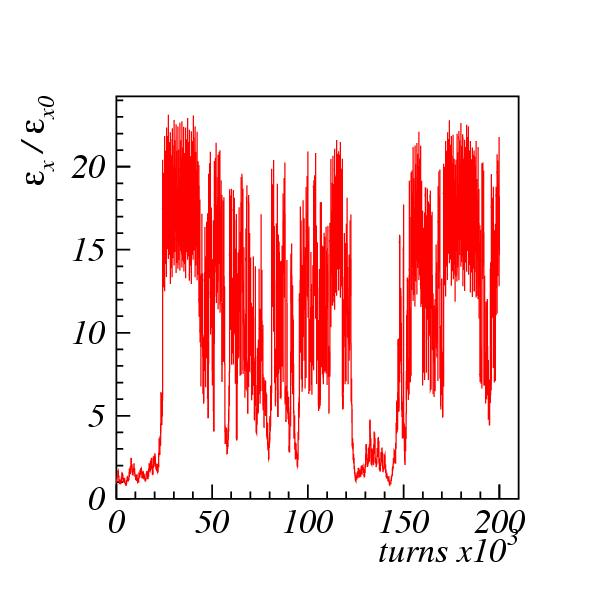
\includegraphics[width=0.5\columnwidth]{Step8_trapping_SIMPSONS.jpg}
        \caption{Step8.}
        \label{fig:step8_s}
\end{figure}

\section{Step 9: Benchmarking of RMS $\epsilon_x$ evolution in $5 \cdot 10^5$ $Q_s$ = 1/1000 for $Q_x$ = 4.3604}

\begin{figure}[!htb]
        \centering
        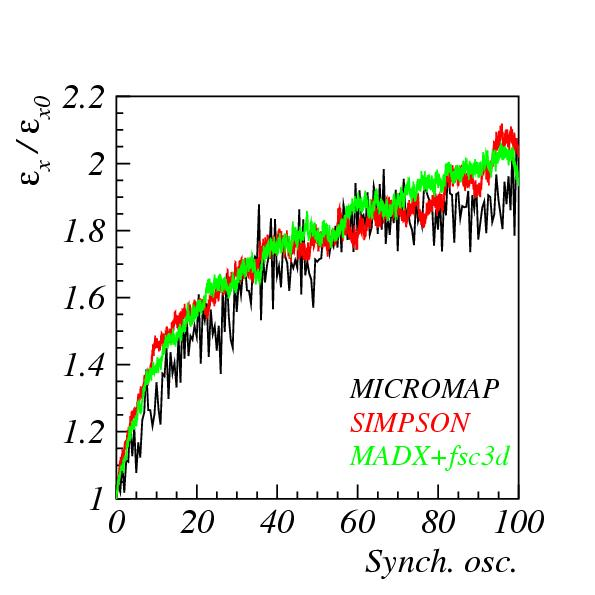
\includegraphics[width=0.5\columnwidth]{Step9_emittance.jpg}
        \caption{Step9.}
        \label{fig:step9}
\end{figure}

\end{document}
